\documentclass[twoside,a4paper,12pt,openany]{book}

\usepackage[spanish]{babel}
\usepackage[utf8]{inputenc}
\usepackage{geometry}
\usepackage{makeidx}
\usepackage{graphicx}
\usepackage{subfigure}
\usepackage{subfig}
%\usepackage[Bjornstrup]{fncychap}
\usepackage{a4wide}
\usepackage{named}
\usepackage[table]{xcolor}
\usepackage{listings}
\usepackage{pdfpages}
\usepackage{appendix}
\usepackage{amsmath}
\usepackage{amsfonts}
%\usepackage{media9}
%\usepackage{hyperref}
\usepackage{url}
\usepackage{cite} % para contraer referencias



% From texlive-science
\usepackage{algorithm}
\usepackage{algorithmic}

%\DeclareGraphicsExtensions{.jpg,.pdf,.png,.ps}
\usepackage{color}
\definecolor{gray97}{gray}{.97}
\definecolor{gray75}{gray}{.75}
\definecolor{gray45}{gray}{.45}

\pagestyle{headings}
\geometry{a4paper, left=3.5cm, right=2cm, top=3cm, bottom=2cm, headsep=1.5cm}

\widowpenalty=10000
\clubpenalty=10000
\hyphenpenalty=10000
\tolerance=10000
%Para que no corte las palabras al final de la linea.

% Latex command para crear listas sin espacio entre
% un item y otro.
\newenvironment{packed_item}{
\begin{itemize}
  \setlength{\itemsep}{1pt}
  \setlength{\parskip}{0pt}
  \setlength{\parsep}{0pt}
}{\end{itemize}}

% Latex command para crear listas umeradas sin 
% espacio entre un item y otro.
\newenvironment{packed_enum}{
\begin{enumerate}
  \setlength{\itemsep}{1pt}
  \setlength{\parskip}{0pt}
  \setlength{\parsep}{0pt}
}{\end{enumerate}}

% Configuracion del entorno lstlistings

\definecolor{dkgreen}{rgb}{0,0.6,0}
\definecolor{gray}{rgb}{0.5,0.5,0.5}
\definecolor{mauve}{rgb}{0.58,0,0.82}

\lstset{frame=tb,
  language=C++,
  aboveskip=3mm,
  belowskip=3mm,
  showstringspaces=false,
  columns=flexible,
  basicstyle={\small\ttfamily},
  numbers=none,
  numberstyle=\tiny\color{gray},
  keywordstyle=\color{blue},
  commentstyle=\color{dkgreen},
  stringstyle=\color{mauve},
  breaklines=true,
  breakatwhitespace=true,
  tabsize=3
}

% minimizar fragmentado de listados
\lstnewenvironment{listing}[1][]
{\lstset{#1}\pagebreak[0]}{\pagebreak[0]}

\lstdefinestyle{consola}
{basicstyle=\scriptsize\bf\ttfamily,
backgroundcolor=\color{gray75},
}

\lstdefinestyle{C}
{language=C,
}

\makeindex

\begin{document}

\thispagestyle{empty}

\baselineskip 1.35\baselineskip

\vspace{2cm}

\begin{figure}[htb]
  \centerline{\resizebox{.60\textwidth}{!}{
\includegraphics{img/logo_urjc}}}
\end{figure}

\begin{center}
  {\Large {\bf Grado en Ingeniería en Telemática}}
  \vspace{5mm}
 
  {\large {Escuela Técnica Superior de Ingeniería Telecomunicación}}
  \vspace{5mm}

  {\large {Curso académico 2017/2018}}

  \vspace{1cm}

  {\large {\bf Trabajo Fin de Grado}}

  \vspace{2cm}

  {\large {Robot submarino OpenROV y ROS\\[1cm] }}

  \vspace{5cm}
  {\bf Autor}: Saúl Ibáñez Cerro
  
  {\bf Tutor}: Francisco Martín Rico 
\end{center}

\clearpage
\newpage{\pagestyle{empty}\cleardoublepage}
\thispagestyle{empty}

\vspace{5cm}
\makebox[15cm][r]{
  \begin{tabular}{ll}
  \emph{A}
  \end{tabular} 
}

\clearpage
\newpage{\pagestyle{empty}\cleardoublepage}
\thispagestyle{empty}

\vspace{5cm}
\textbf{\huge{Agradecimientos}}\\

Primero, quiero agradecer a mis padres todo el esfuerzo que han realizado por mí, por haberme apoyado durante toda mi vida académica, muchas gracias por estar siempre ahí, por quererme y por animarme cuando más lo necesitaba.
También quiero agradecer al ``enano'' de mi corazón, mi hermano, con el que siempre he podido hablar de mis quebraderos de cabeza.
Por supuesto, también merece una mención especial mi pareja, Paula, no sé si hubiera podido con la presión y desánimos si no fuera por ella. Me ha ayudado más que nadie, le debo muchísimo.
Otro apoyo muy grande que he tenido han sido los padres de mi novia, que han estado siempre ahí cerca ayudándome.
A mis abuelos por apoyarme y a todos los amigos y compañeros que me han ayudado durante toda esta etapa.
Para finalizar quiero mostrar mi gratitud a un profesor que me ha marcado, por la forma de enseñar y mostrarnos su asignatura, el profesor de robótica, Francisco Martín, al que también agradezco darme la oportunidad de hacer un TFG distinto.

Muchas gracias a todos. Todos los éxitos que consiga en la vida, serán en parte gracias a vosotros.

\clearpage
\newpage{\pagestyle{empty}\cleardoublepage}

%%%%%%%%%% RESUMEN %%%%%%%%
\newpage{\pagestyle{empty}\cleardoublepage} 
%\input{resumen}

                                %\pagenumbering{roman}

                                %\setcounter{page}{1}
\frontmatter
\tableofcontents

\listoffigures
                                %\setcounter{page}{1}
                                %\pagenumbering{arabic}
%\listoftables

\mainmatter

% Init counter page
\setcounter{page}{1}

% Capitulo 1
\chapter{Introducción}

En este capítulo se explicará el concepto de robótica móvil\cite{RoboticaMovil}.
También se comentarán los robots submarinos, ya que en este proyecto, trataremos sobre uno de ellos, OpenROV.
Hablaremos sobre ROS (Robot Operating System), que tiene un conjunto de herramientas y atajos que facilitan la comunicación y operabilidad de los robots, ya que en uno de los capítulos del proyecto, se expondrá la integración de este framework en el ROV.
Para finalizar se describirá la estructura de la memoria y de los apartados que conlleva.

\section{Robótica móvil}
\label{cap:roboticamovil}
Generalmente las aplicaciones robóticas se centraban en los sectores manufactureros más desarrollados para la producción masiva: industria del automóvil, transformaciones metálicas, etc.

A principios de los años sesenta se introducen en la industria los robots manipuladores como un elemento más del proceso productivo. Los trabajos desarrollados por los robots manipuladores consistían frecuentemente en tareas repetitivas.

Un robot móvil puede moverse sobre entornos no estructurados, de los cuales, no se posee conocimiento. Esto lo realiza mediante la interpretación de los datos obtenidos a través de los sensores y del estado actual del vehículo. 

En general se considera que existen tres clases de robots:
\begin{itemize}
\item \textbf{Industriales}, son los de mayor difusión en tareas de alcance económico, formados por una estructura mecánica articulada, que se mueve adoptando distintas configuraciones por las órdenes recibidas de un equipo de control, generalmente, un microprocesador.
\item \textbf{Médicos}, se diseñan prótesis inteligentes para la rehabilitación de disminuidos físicos. Se procura que estas prótesis tengan la estética correspondiente a la extremidad perdida.
\item \textbf{Móviles}, tienen una plataforma mecánica dotada de un sistema de locomoción capaz de navegar a través de un determinado ambiente de trabajo.

Este tipo de robots estan dotados de un sistema de locomoción, el cual, es capaz de navegar en distintos entornos de trabajo. La locomoción puede estar diseñada con patas (equilibrio estático o dinámico) o con ruedas, que al final, son más eficientes que las piernas y son estáticamente estables. 

El mayor inconveniente de la locomoción es el desplazamiento a un lugar concreto, planificar las trayectrias y seguir la una determinada trayectoria puede resultar imposible para algunos robots.

Un robot móvil autónomo se caracteriza por una conexión inteligente entre las operaciones de percepción y actuación.
\begin{itemize}
  \item \textbf{Percepción}, es la capacidad del robot móvil para gestionar la información obtenida a través de los sensores (u otros medios) con el objetivo de lograr una navegación global o local.
   \begin{itemize}
    \item Navegación global es aquella que se apoya en mapas (SLAM). Existen varios tipos, entre los que encontramos:
      \begin{enumerate}
	\item Planificación de los caminos (planes clásicos (secuencia de subobjetivos) y planes con recursos (por donde se le recomienda ir)).
	\item Navegación basada en mapas.
	\item Listas de caminos, grafos de objetos o balizas.
	\item Grafos de visibilidad.
	\item Diagramas de Voroni.
	\item Descomposición en celdas.
	\item Planificación como descenso del gradiente.
      \end{enumerate}
    \item Navegación local es aquella que puede navegar si un mapa, y las tecnologías más usadas en ellas son:
      \begin{enumerate}
	\item Método de velocidad y curvatura (CVM), el cual, trabaja añadiendo restricciones al espacio de velocidad y escogiendo un punto del espacio que satisfaga todas las restricciones y maximice una función objetivo.
	\item Método de carriles y velocidad (LVM), esta tecnología, divide el entorno en carriles para decidir cual es el mejor camino a seguir.
	\item Método de fuerzas virturales (VFF), tanto los obstaculos como el destino ofrecen un tipo de fuerza, repulsiva y atractiva respectivamente. Al final, el movimiento del robot está gobernado por el sumatorio vectorial de dichas fuerzas.
      \end{enumerate}
   \end{itemize}
  \item \textbf{Actuación}, el robot móvil tiene que de decidir que acción es la idónea en cada momento, dependiendo del entorno y de su estado.
\end{itemize}
\end{itemize}


\section{Robots Submarinos}
\label{cap:Robots Submarinos}
En este apartado, se hará una breve introducción sobre los robots submarinos (en este trabajo nos centraremos en uno de ellos, OpenROV 2.8\footnote{https://www.openrov.com/products/openrov28/}) y donde pueden resultar de mayor utilidad.

El mundo de los robots submarinos ROV (\textit{Remote Operated Vehicle} o vehículo de operación remota) sigue creciendo año tras año. El 71\% de la superficie de la Tierra está cubierta de océanos y sin embargo, solo se ha mapeado el 5\% del suelo oceánico.

Durante los últimos años, el uso de robots submarinos ha aumentado rápidamente, ya que este vehículo puede operar en áreas más profundas y más peligrosas, a los cuales los humanos no podemos llegar. Este tipo de robot se pueden utilizar para el área de la pesca, control submarino de contaminación, manipulsación y limpieza del océano, así como de sitios nucleares.

Se trata de un área de diversas aplicaciones en el mundo real, ya que permite y facilita la exploración, estudios científicos de zonas inexploradas, la búsqueda y el rescate de navíos.

Podriamos diferenciar las diferentes áreas potenciales en las cuales tienen una aplicación como:

  \begin{itemize}
  \item \textbf{Ciencia}
    \subitem Generación de mapas del suelo marino.
    \subitem Rápida respuesta a eventos eceanográficos y geotérmicos.
    \subitem Muestreo geológico
  \item \textbf{Militar}
   \subitem Búsqueda y eliminación de minas submarinas. 
   \subitem Reconocimiento de rutas, áreas y zonas. 
   \subitem Vigilancia. 
   \subitem Búsqueda y rescate. 
   \subitem Adquisición de objetos. 
   \subitem Seguridad en las rutas. 
   \subitem Soporte en el desarrollo de la situación. 
   \subitem Soporte en la preparación del campo de batalla. 
  \item \textbf{Minería oceánica e industria del petróleo}
    \subitem Estudio del océano y evaluación de recursos.
    \subitem Construcción y mantenimiento de estructuras submarinas.
  \item \textbf{Otras}
    \subitem Inspección del casco en los barcos.
    \subitem Inspección de plantas nucleares.
    \subitem Instalación e inspección de cables. 
    \subitem Rutas turísticas bajo el mar.
    \subitem Etc.
 \end{itemize}

\begin{figure}[hbtp]
  \begin{center}
    \subfigure[Robot Deep Trekker]{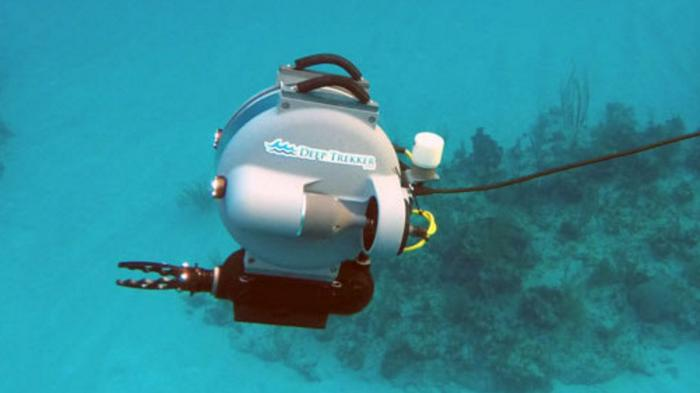
\includegraphics[width=6cm,height=5cm]{img/cap1/submarino1}}
    \subfigure[Robot OpenROV]{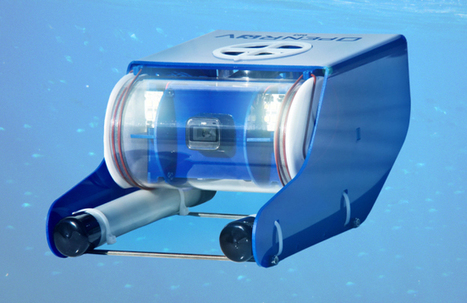
\includegraphics[width=6cm,height=5cm]{img/cap1/submarino2}}
  \end{center}
  \caption{Robots submarinos}
  \label{fig:submarino}
\end{figure}
  
\section{ROS}
\label{cap:ROS}

Sistema Operativo de Robots (en inglés \textit{Robot Operating System, ROS}\cite{ros}) es un framework para el desarrollo de software para robots. 

Implementaremos ROS en el robot submarino ya que es el framework por excelencia para el desarrollo de las aplicaciones robóticas. Contiene algoritmos implementados, además de proporcionar una arquitectura distribuida. No hace falta que los nodos de ROS interactuen en el mismo sistema ni que deban ser de la misma arquitectura, por eso es una gran ventaja utilizarlo en la tecnología de OpenROV. 

ROS provee los servicios estándar de un sistema operativo tales como abstracción del hardware, control de dispositivos de bajo nivel, implementación de funcionalidad de uso común, paso de mensajes entre procesos y mantenimiento de paquetes. Está basado en una arquitectura de grafos donde el procesamiento toma lugar en los nodos que pueden recibir, mandar y multiplexar mensajes de sensores, control, estados, planificaciones y actuadores, entre otros.

ROS tiene dos partes básicas: la parte del sistema operativo, ROS, y una suite de paquetes aportados por la contribución de usuarios que implementan la funcionalidad, como localización y mapeo simultáneo, planificación, percepción, simulación, etc.

ROS es OpenSource bajo términos de licencia BSD. Esta licencia permite libertad para uso comercial e investigador.

ROS utiliza de topics como modelo de comunicación entre procesos, a los que se les nombra como nodos. A continuación se detallan los conceptos principales de ROS:
\begin{enumerate}
 \item \textbf{Master}. Proporciona el registro de nombre. Sirve para encontrar los nodos, intercambiar mensajes e invocar servicios. 
 Para ejecutar el ROS Master, utilizaremos el comando:
  \renewcommand{\lstlistingname}{}
  \begin{lstlisting}[caption=roscore, label={lst:roscore}]
    $ roscore
  \end{lstlisting}
  
  Y se visualizará lo siguiente:
  
  \begin{figure} [hbtp]
  \begin{center}
    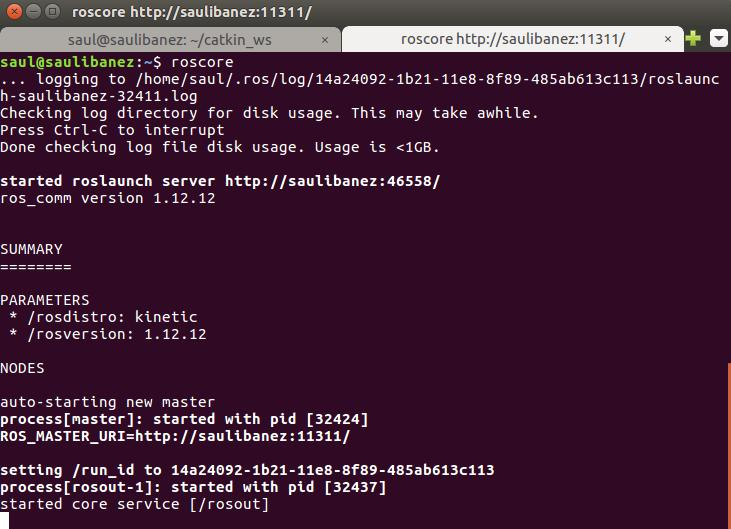
\includegraphics[width=12cm]{img/cap1/roscore}
  \end{center}
  \caption{Roscore}
  \label{fig:roscore}
  \end{figure}
  
  A partir de ahora, el sistema ya sabe donde encontrar los comandos para ejecutar ROS.
  \item \textbf{Nodos (Node)}. Son procesos de comunicación. Por ejemplo, un nodo controla la cámara, otro nodo controla los motores, etc. En general, los nodos son ejecutables que se comunican con otros procesos, a los que denominamos tópicos.
  \item \textbf{Mensajes}. Son estructuras de datos compuestos (integer, float, string, arrays, etc).
  \item \textbf{Tópicos (Topics)}. Es un canal de comunicación para transmitir los datos, el cual uiliza el modo de suscriptor y publicador. Puede existir varios publicadores para un único tópico, al igual que un nodo puede publicar y/o suscribirse a múltiples tópicos.
  Se transimite utilizando la tecnología de TCP/IP o UDP.
\end{enumerate}


\section{Estructura de la memoria}
\label{cap:estructuradelamemoria}
En este documento se describen los aspectos más relevantes del desarrollo y montaje del robot. La memoria esta dividida en 6 capítulos. 
El primer capítulo, Introducción, se ha realizado una presentación de los robots móviles. En el segundo capítulo se define el problema y se establecen los objetivos. El montaje del robot, el entorno y las herramientas utilizadas se especifica en el tercer capítulo. En el siguiente capítulo, el cuarto, se mostrará la integración del OpenROV con ROS. En el quinto capítulo se expondrán una serie de videos comprobando el funcionamiento del OpenROV, y en el último, el sexto, expondré las conclusiones del trabajo.


% Capitulo 2
\chapter{Objetivos y Metodología}
\label{cap:objetivos}
Tras haber presentado el contexto en el que se desarrollará este proyecto, en este capítulo se fijarán los objetivos y se expondrán los requisitos para llegar a la solución.
\section{Descripción del problema y requisitos}
\label{sec:descripciondelproblema}

El fondo oceánico es uno de los grandes misterios de la actualidad. La mayor parte del suelo oceánico no ha sido explorado, y eso supone un gran problema. Con este robot podremos rozar un poco este mundo submarino tan fascinante, e intentar descubrir algunas de las magníficas maravillas que esconde.

El robot contiene una cámara de alta resolución que permite visualizar el suelo oceánico. Cuando la visión de la cámara sea baja o nula, precisaremos de las luces y los láseres incorporados, con ellos, podremos visualizar mejor el entorno y saber la distancia a la que se encuentren los objetos, plantas o animales. 

Los requisitos indispensables para realizar el proyecto son:
\begin{enumerate}
\item \textbf{Impermeabilidad} durante todo el proceso de sumersión
\item \textbf{Conectividad.} El robot puede alcanzar una distancia de 100m sin que pierda señal.
\item \textbf{Duración de las baterías.} El robot debe permanecer activo durante 6 horas. 
\item \textbf{Web Cockpit.} Control del funcionamiento del robot.
\end{enumerate}

\section{Objetivo del proyecto}
\label{sec:objetivos}

El objetivo del proyecto es el montaje, configuración del software de ROV y ROS, y unas pruebas de campo del robot submarino OpenROV. 
\\Se montará de cero el robot submarino, utilizando los materiales dados por la comunidad de OpenROV. A la placa de OpenROV se le instalará un PLC para la comunicación del robot con el portátil y otra placa BeagleBone, que llevará implantado el software necesario para la comunicación y funcionamiento con el robot.
\\Además, se implantará una biblioteca de ROS dentro de OpenROV para que también se pueda comunicar a través del framework de robótica más famoso. Con esta biblioteca instalada y ejecutando el ROS Master en el portátil, se podrá realizar una comunicación.

\section{Metodología de desarrollo}
\label{sec:metodologiadedesarrollo}

En el desarrollo del sistema descrito, el modelo de ciclo de vida utilizado ha sido el modelo Modelo en cascada\cite{cascada}.

Es un proceso secuencial, fácil de desarrollo en el que los pasos de desarrollo son vistos hacia abajo (como en una cascada de agua) a través de las fases de análisis de las necesidades, el diseño, implantación, pruebas (validación), la integración, y mantenimiento. 

Los principios básicos del modelo de cascada son los siguientes:
\begin{figure} [hbtp]
  \begin{center}
    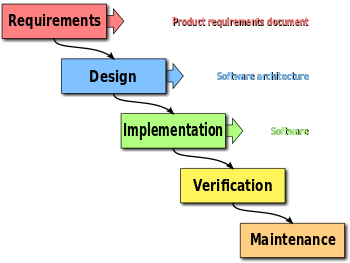
\includegraphics[width=11cm]{img/cap2/Waterfall_model}
  \end{center}
  \caption{Modelo en cascada.}
  \label{fig:Waterfall_model}
\end{figure}

\begin{itemize}
\item El proyecto está dividido en fases secuenciales.
\item Se hace hincapié en la planificación, los horarios, fechas, presupuestos y ejecución de todo un sistema de una sola vez.
\item Se mantiene un estricto control durante la vida del proyecto a través de la utilización de una amplia documentación escrita.
\end{itemize}

\section{Plan de trabajo}
\label{sec:plandetrabajo}

Para poder abordar el problema se han marcado una serie de objetivos a completar. Dichos hitos son los siguientes:

\begin{enumerate}
\item Estudio, comprensión y montaje del OpenROV 2.8.
\item Una vez terminado el montaje, se realizará la conexión del ROV para comunicarse con el portátil.
\item \textbf{Fase de pruebas}, se probará el robot en distintos entornos para comprobar su funcionamiento.
\item Estudio y comprensión de los paquetes de ROS roslibjs\footnote{http://wiki.ros.org/roslibjs} (biblioteca de JavaScript para interactuar con ROS) y rosbridge\footnote{http://wiki.ros.org/rosbridge\_suite} (envía mensajes JSON para comunicarse con ROS a través de websocket, además, controla la ejecución de los nodos).
\item Integración de ROS y OpenROV.
\end{enumerate}

% Capitulo 3
\chapter{Plataforma OpenROV}
\label{cap:plataformaOpenROV}

\section{Robot Submarino OpenROV}
\label{cap:Robot Submarino OpenROV}
La robótica submarina lleva desarrollándose desde mediados de los años sesenta, aunque fuera una realidad desconocida para el gran público. Los robots submarinos costaban millones y tenían el tamaño de un todoterreno. Un robot con una cámara que se retransmite en directo a una página web. Su principal virtud es que OpenROV\cite{openrov} funciona con código abierto.

En general, sus características entran dentro de los parámetros presentados a continuación:

  \begin{itemize}
  \item \textbf{Cámara web de alta definición para video en vivo HD} Se transmite vídeo de alta definición a un portátil a través de un cable trenzado de dos hilos.
  \item \textbf{Tres servomotores} Se utilizan para la movilidad del dispositivo. Son de muy bajo mantenimiento y puedan estar en contacto directamente con el agua.
  \item \textbf{Flotabilidad neutra y altamente maniobrable} El diseño compacto y ligero permite una alta maniobrabilidad utilizando un diseño de tres actuadores. Se puede sumergir a una profundidad de 100 metros.
  \item \textbf{Interfaz web fácil de usar} En ella se puede manipular la cámara, los láser, focos y motores. No necesita conexión a Internet, ni hay necesidad de instalar un software.
  \item \textbf{Soporte de la comunidad de OpenROV}.
  \end{itemize}

\begin{figure}[hbtp]
  \begin{center}
    \subfigure[OpenROV parte frontal]{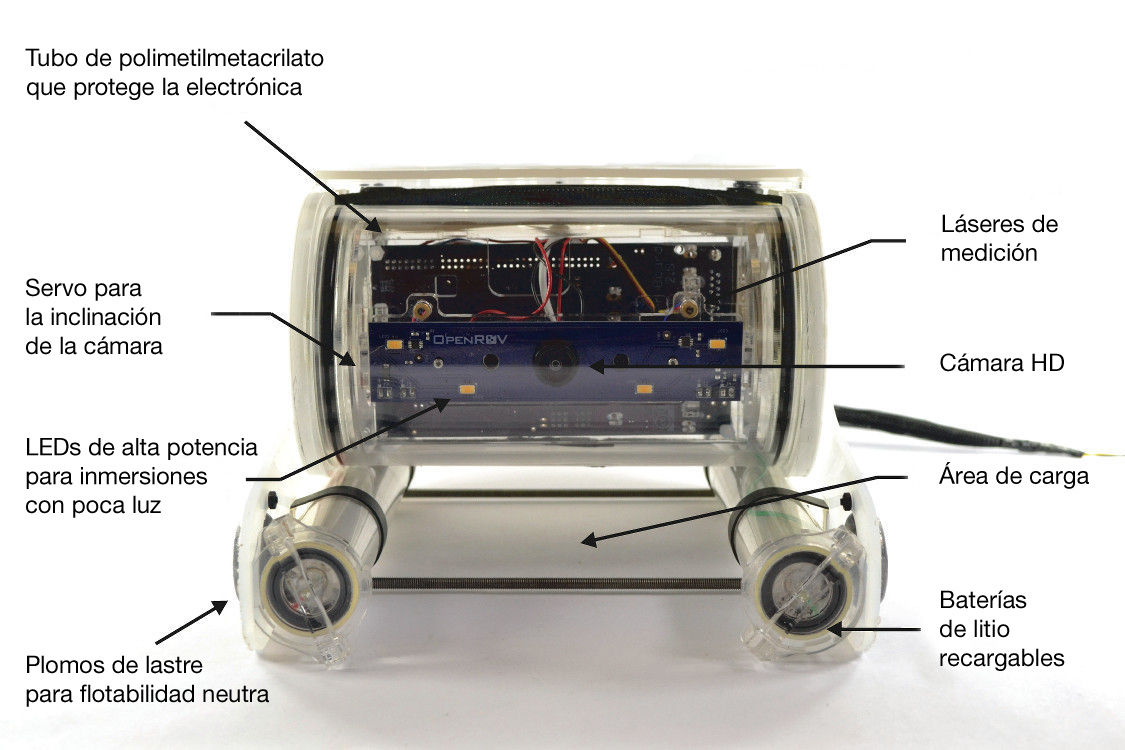
\includegraphics[width=6cm,height=5cm]{img/cap3/ROV_frontal}}
    \subfigure[OpenROV parte trasera]{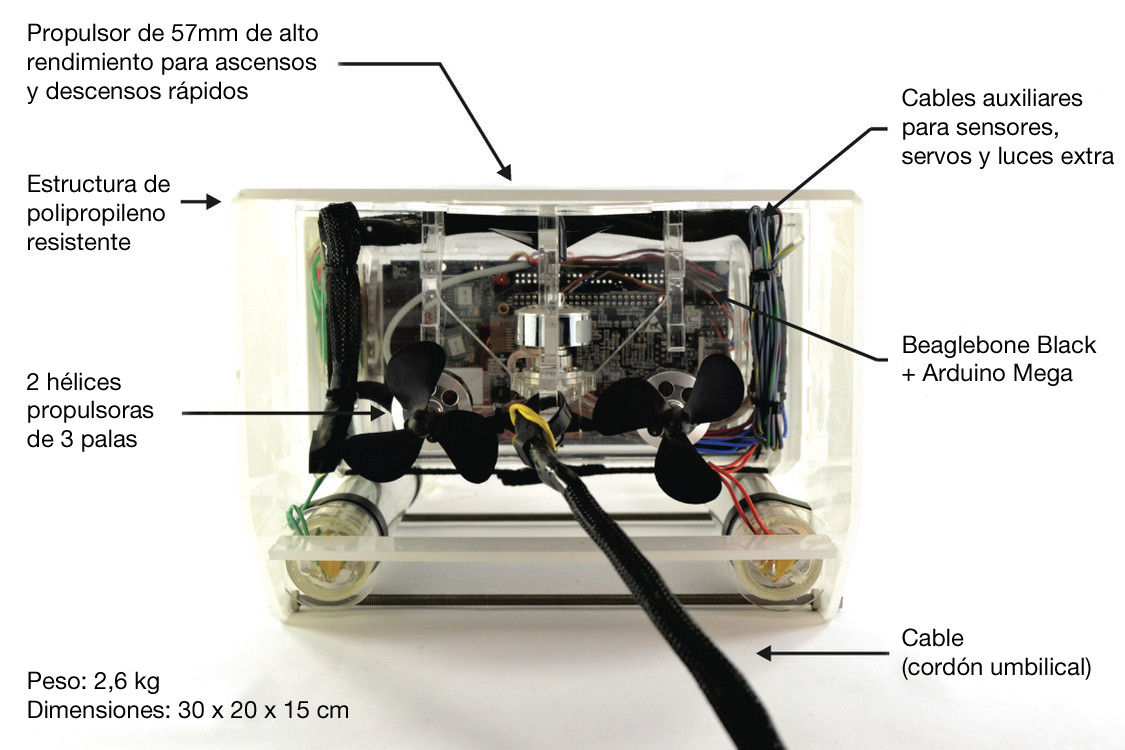
\includegraphics[width=6cm,height=5cm]{img/cap3/ROV_trasera}}
  \end{center}
  \caption{OpenROV}
  \label{fig:ROV-ej}
\end{figure}

\section{Estructura y Montaje}
\label{cap:montaje}

En esta sección se va a describir cada paso del montaje del robot, desde el montaje de cada uno de los chasis hasta la electrónica, de la cual tendremos que soldar los elementos.

\subsection{Estructura de OpenROV}
\label{subsec:EstructuraOpenROV}

Antes de comenzar con el montaje de la estructura, la cámara y el chasis del ROV, se necesitarán ciertas herramientas para el correcto ensamblaje.

Las herramientas necesarias son: guantes, gafas, cúter, cemento acrílico y pegamento. Una vez hayamos obtenido todos los materiales empezaremos con el montaje.

\begin{figure} [hbtp]
  \begin{center}
    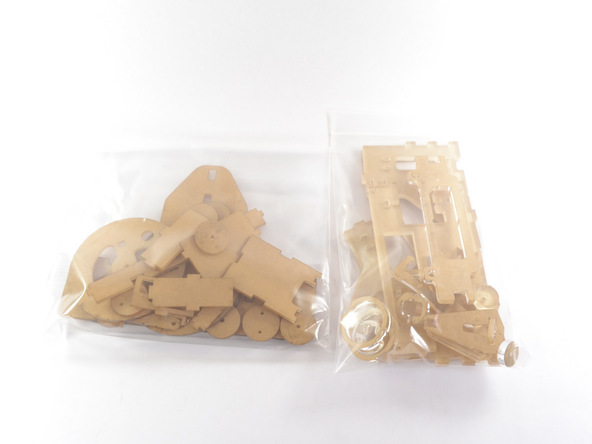
\includegraphics[width=8cm]{img/cap3/3_3/piezas}
  \end{center}
  \caption{Piezas de los chásis.}
  \label{fig:piezas}
\end{figure}

Se separan las piezas para realizar su correcto montaje. Una vez localizadas las piezas para la estructura, se le quitará el papel protector a la pieza, lo cual la dejará de un color trasparente. 
Iremos pegando y dejando secar para que la composición sea la correcta. 
Al final, quedará una estructura como la de la imagen.

\begin{figure} [hbtp]
  \begin{center}
    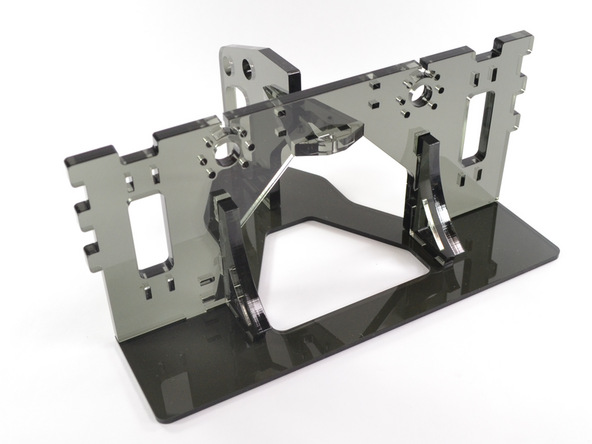
\includegraphics[width=8cm]{img/cap3/3_3/chasis_ppal}
  \end{center}
  \caption{Chasis principal.}
  \label{fig:chasis_ppal}
\end{figure}

Para el montaje de la estructura del soporte de la cámara y el chasis de la electrónica se realizará el mismo procedimiento que en el caso anterior, con un resultado como el de las siguientes fotos:

\begin{figure}[hbtp]
  \begin{center}
    \subfigure[Soporte de la cámara]{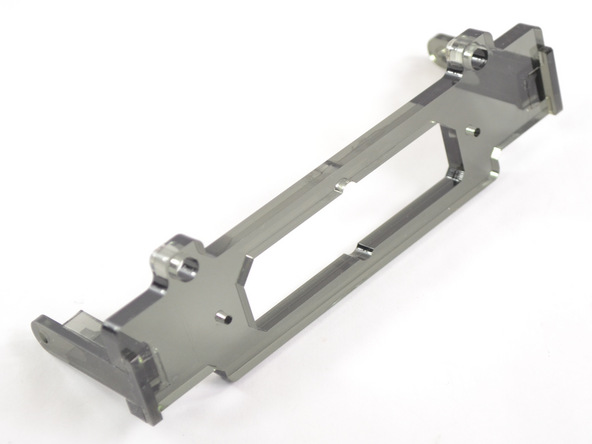
\includegraphics[width=6cm,height=5cm]{img/cap3/3_3/chasis_camara}}
    \subfigure[Chasis de la electrónica]{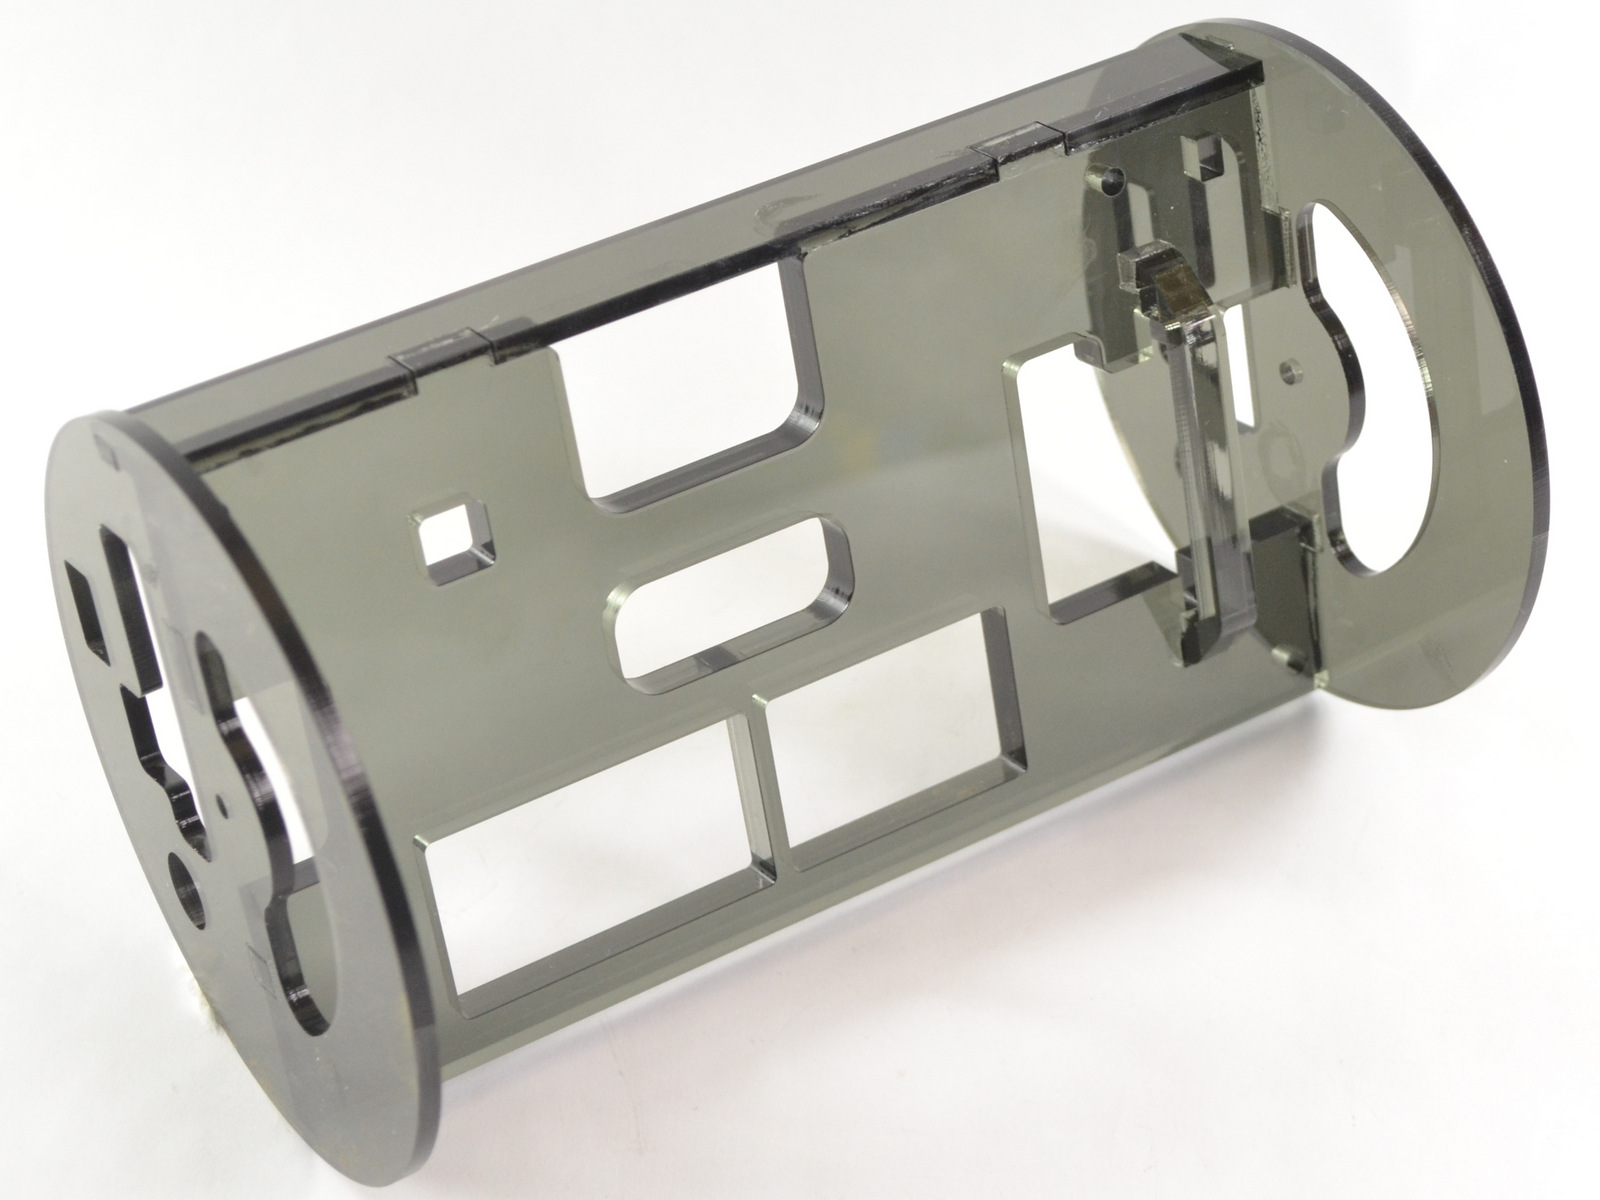
\includegraphics[width=6cm,height=5cm]{img/cap3/3_3/chasis_electronico}}
  \end{center}
  \caption{Soporte de la cámara y electrónica}
  \label{fig:ROV-chasis}
\end{figure}

\subsection{Tapas del chásis}
\label{subsec:tapasChasis}

Al igual  que en el punto anterior, antes de comenzar con el montaje de la tapa, se necesitarán ciertas herramientas para el correcto ensamblaje.

Las herramientas necesarias son: guantes, gafas, cúter, cemento acrílico,  SuperGlue y epoxy (epoxy es un tipo de pegamento que soporta estar en contacto con el agua). Una vez hayamos obtenido todos los materiales empezaremos con el montaje.

En este caso, existen dos tapas. En la primera (la superior), necesitaremos una jeringa proporcionada por la comunidad de OpenROV, la cual utilizaremos para preparar la impermeabilización y el sellado de los componentes software del robot.

En la segunda tapa, está el conector DB-25, el cual, conecta todos los componentes eléctricos a la placa del controlador. Una vez realizado el montaje de la tapa, se pegará en el espacio sobrante el conector DB-25 y se colocarán los cables adecuadamente en el hueco de la tapa. Cuando esté todo debidamente colocado se pegará la tapa superior al montaje realizado, lo cual dejará todo debidamente sellado. Este hueco, se rellenará con el epoxy para que no entre agua por la ranura.

\begin{figure}[hbtp]
  \begin{center}
    \subfigure[Tapa inferior desmontada]{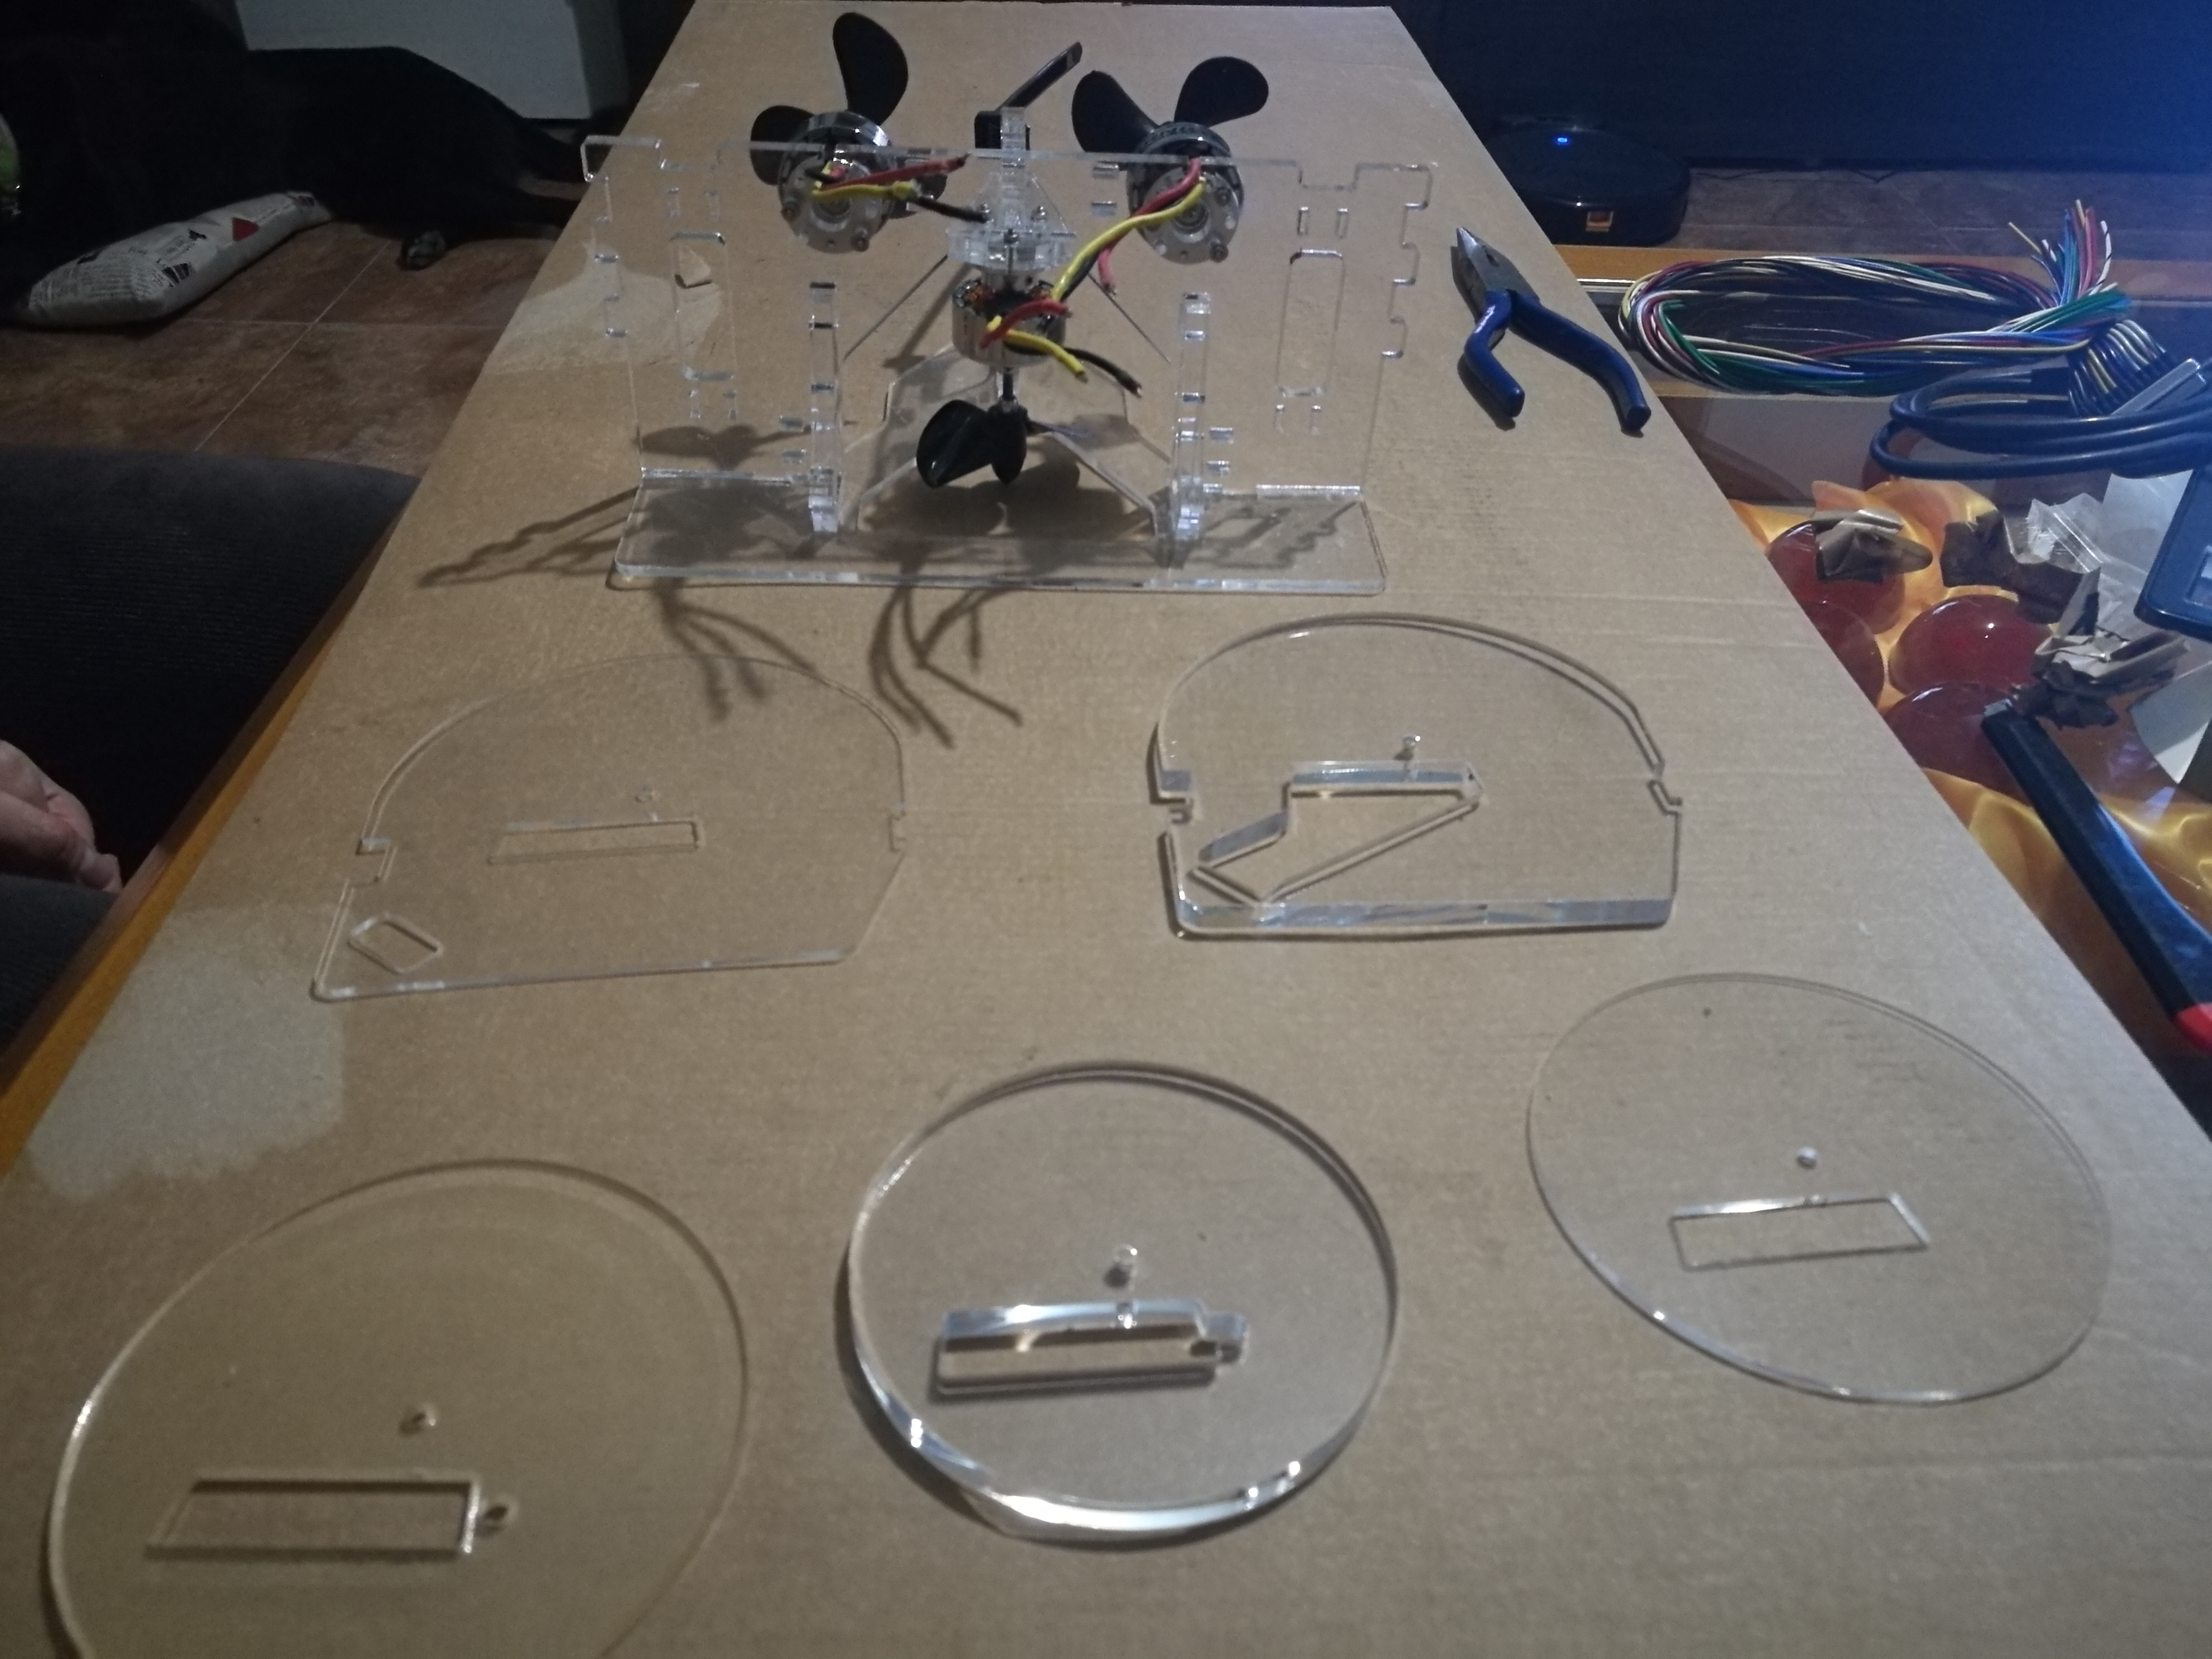
\includegraphics[width=6cm,height=5cm]{img/cap3/3_3/tapa_inf_desmontada}}
    \subfigure[Tapa inferior montada]{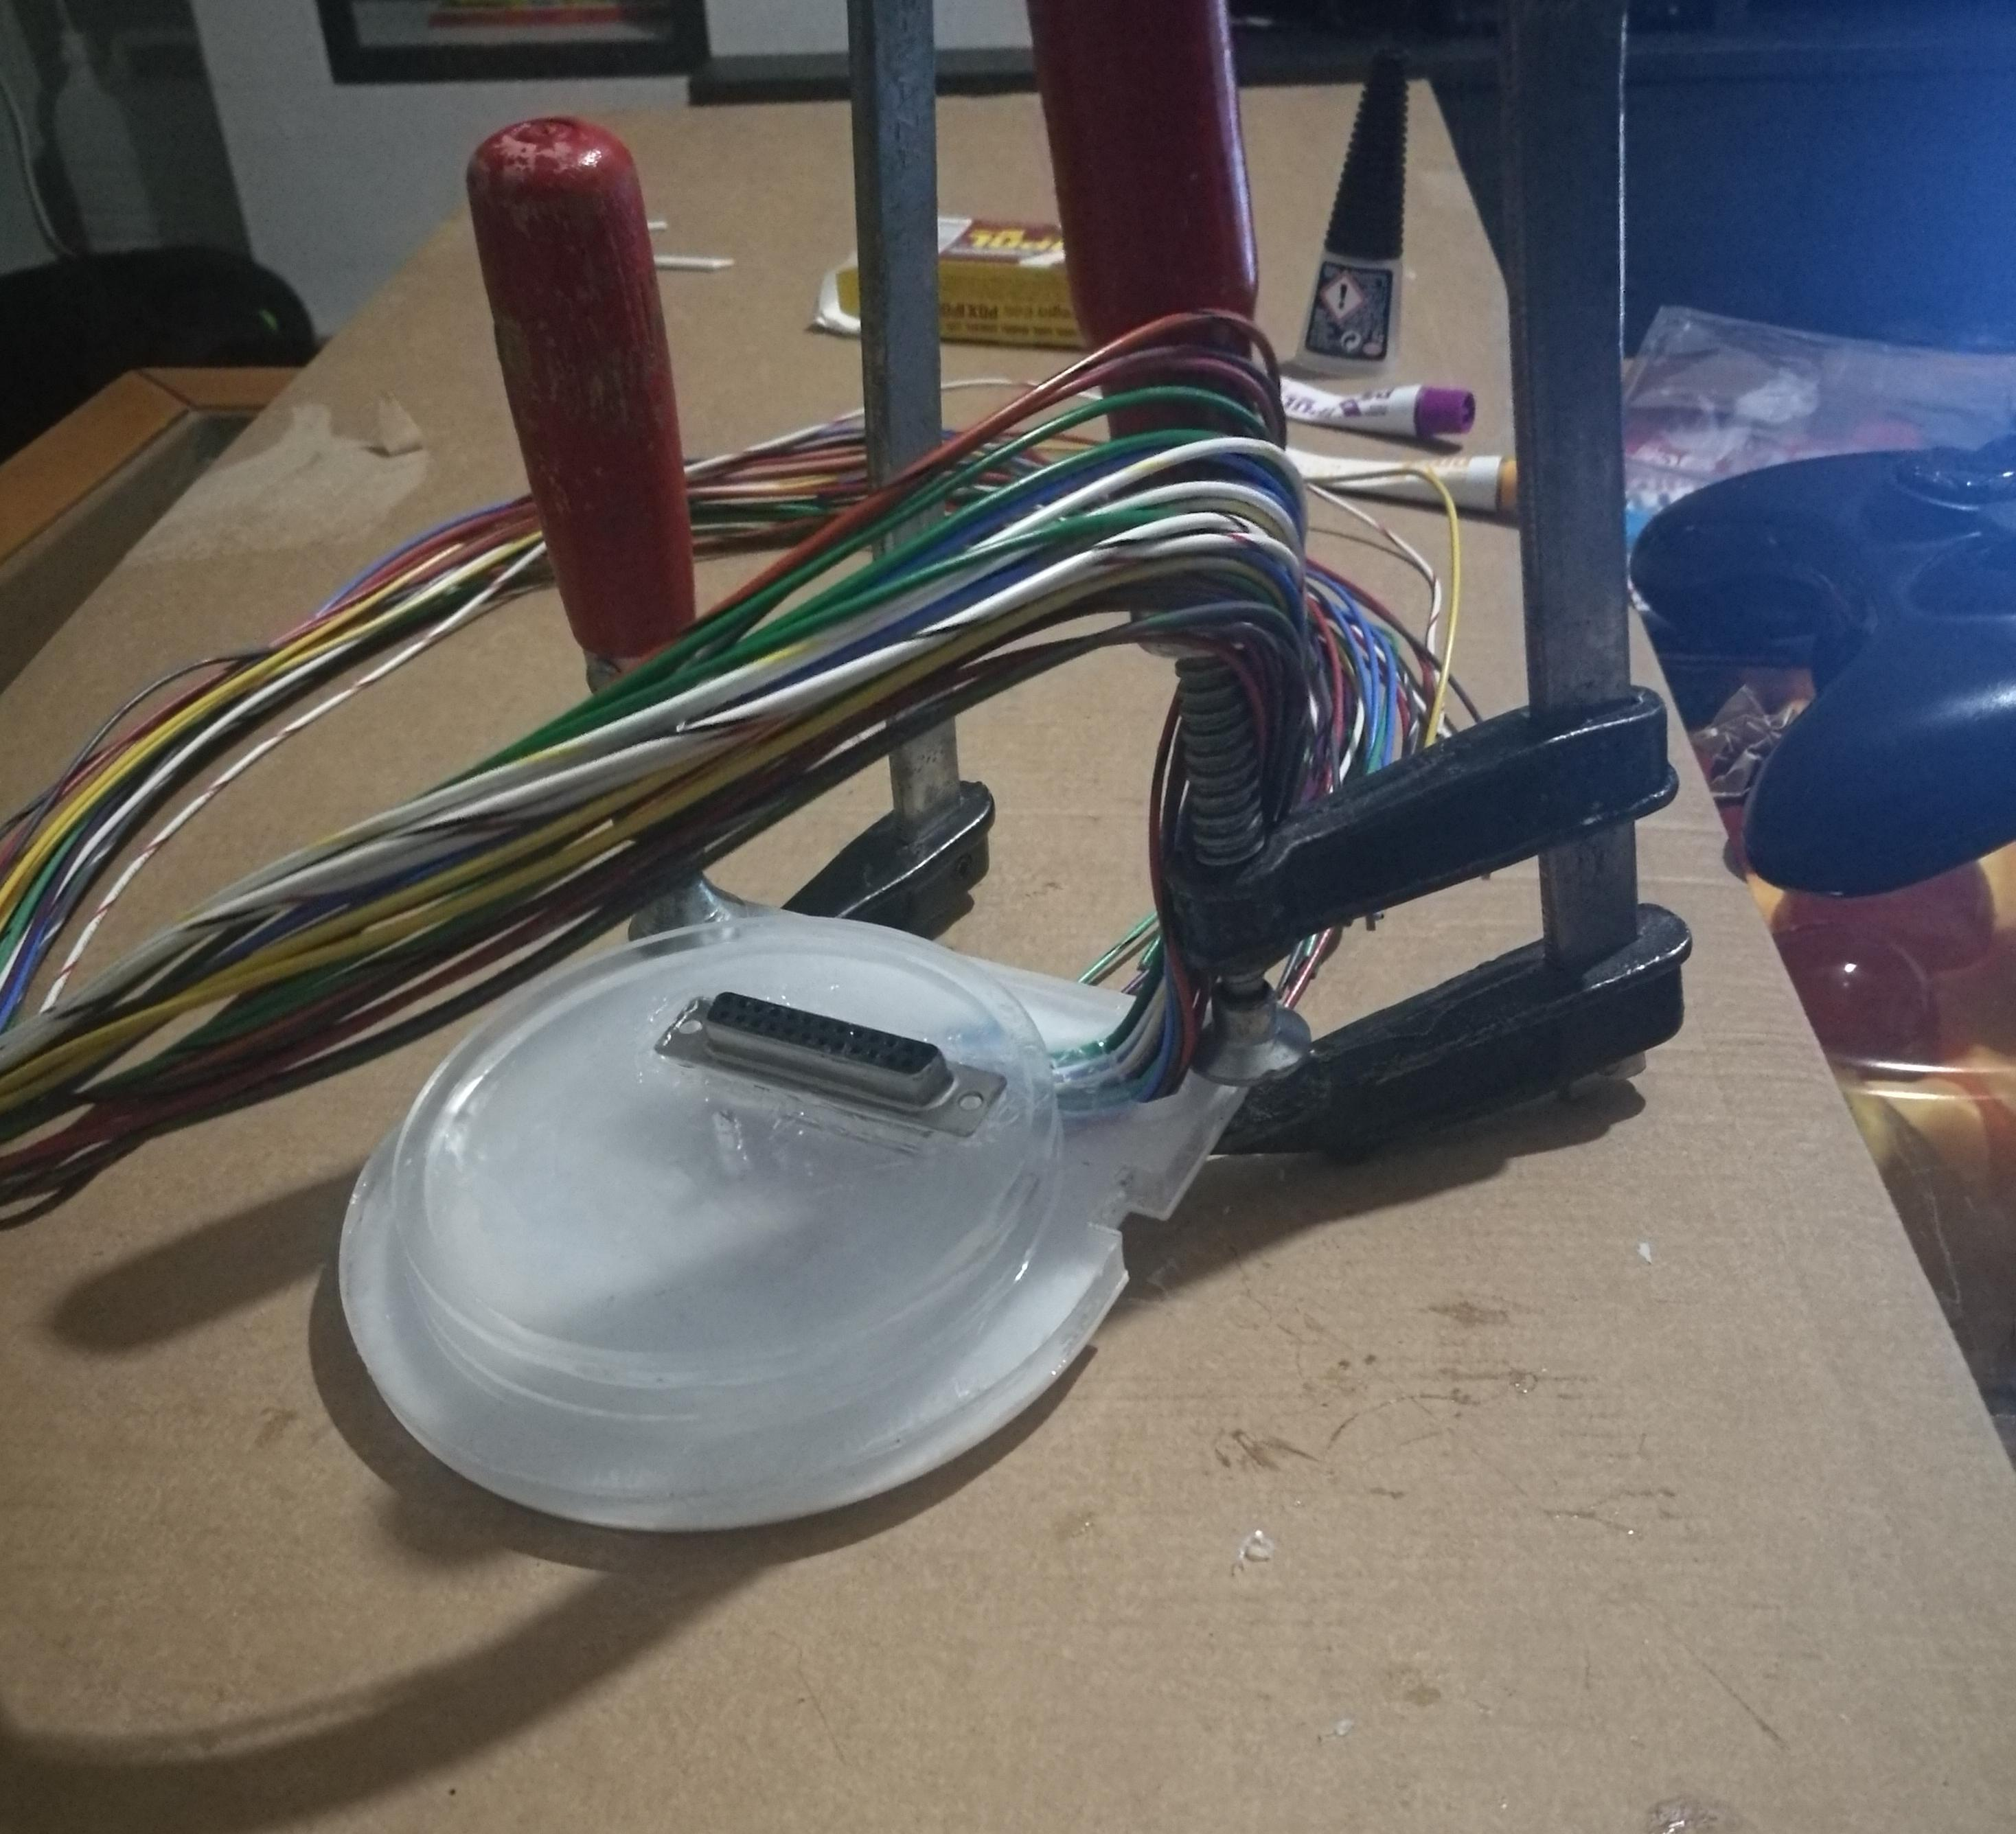
\includegraphics[width=6cm,height=5cm]{img/cap3/3_3/tapa_inf}}
  \end{center}
  \caption{Tapa inferior}
  \label{fig:tapa_iferior}
\end{figure}

\subsection{Electrónica}
\label{subsec:electronica}

Este es el punto crucial del funcionamiento del robot y se necesita especial atención en cada uno de los pasos. 

Al igual que en los apartados anteriores, necesitaremos material especial, entre los que están el soldador, estaño, PLC, BeagleBone, tijeras y destornilladores.

Para empezar, desmontaremos los PLC para sacar el hardware, el cual utilizaremos más adelante.
Uno de los PLC estará interno en el robot, y el otro, será el extremo conector que comunicará el ROV con el portátil.

Continuaremos con el BeagleBone Black (BBB), el cual, es el procesador principal en el ROV. Funciona junto con un Ardunio en el tablero del controlador para controlar las muchas funciones del ROV.

El cable USB del BeagleBone lo utilizaremos más adelante.

Una vez juntos el PLC, el BeagleBone y la placa del ROV, uniremos estos tres elementos para formar el hardware del robot. Se conectará primero la placa del ROV, en la que el conector RJ-45 irá conectado al hardware PLC. Una vez realizada esa conexión, procederemos a implantar en las ranuras el BeagleBone, y atornillaremos para obtener una mejor sujeción, como podemos comprobar en la imagen.

\begin{figure} [hbtp]
  \begin{center}
    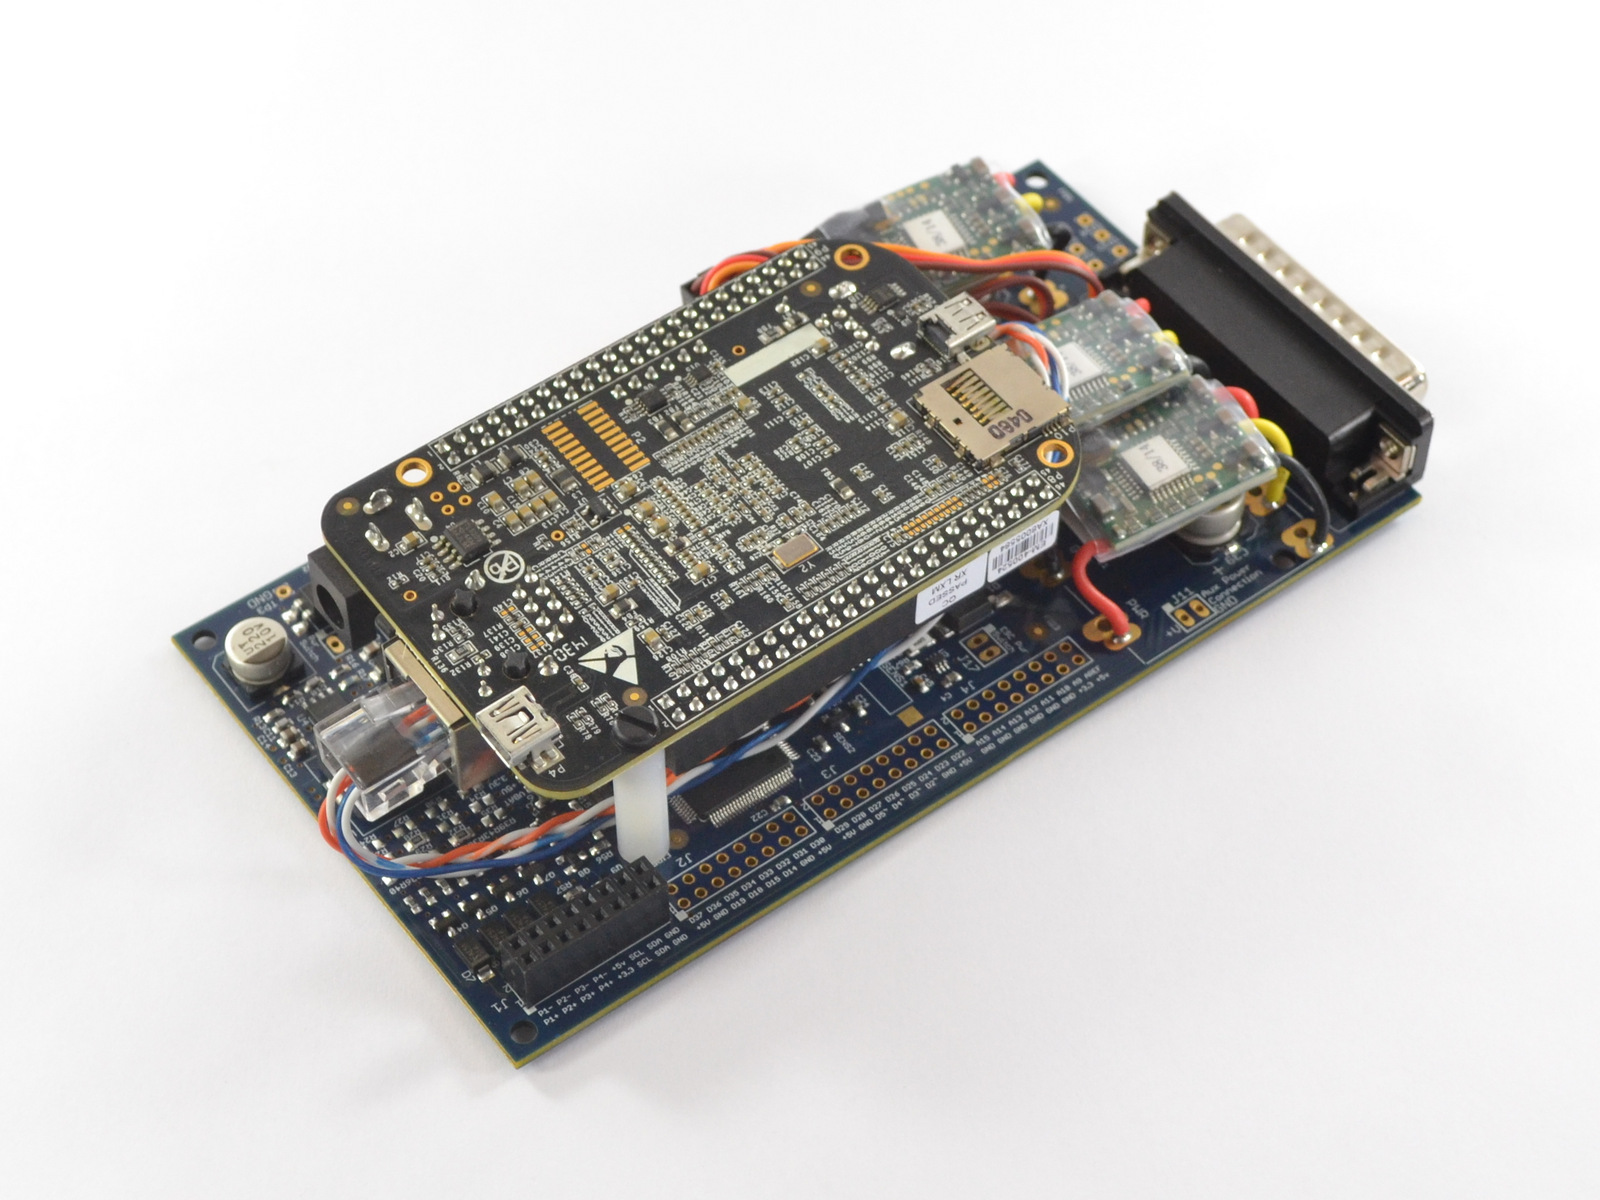
\includegraphics[width=8cm]{img/cap3/3_3/electronica}
  \end{center}
  \caption{Raspberry Pi + PLC + BeagleBone}
  \label{fig:electronica}
\end{figure}

Después, conectaremos el servo al chasis, el cual va a servir para mover la cámara verticalmente. Hay que asegurarse de que quede centrado.

Continuaremos con la soldadura de los láser y unos cables a la placa de video del ROV.

\begin{figure} [hbtp]
  \begin{center}
    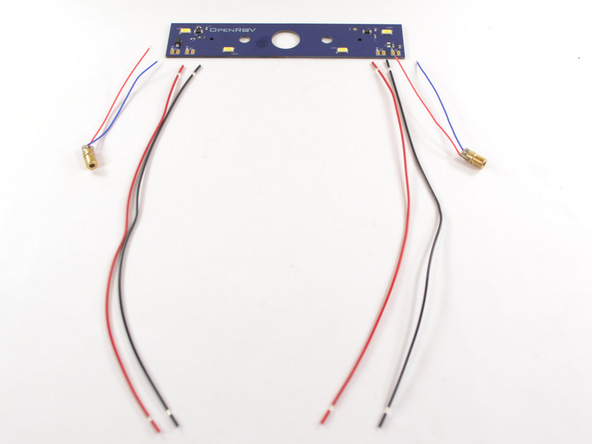
\includegraphics[width=8cm]{img/cap3/3_3/electronica_camara}
  \end{center}
  \caption{Electrónica de la cámara}
  \label{fig:electronica_camara}
\end{figure}

Cuando estén debidamente soldados, se colocará el chasis de la cámara, junto con lo que acabamos de soldar y la cámara. A estos tres elementos los juntaremos con tornillos y tuercas. Para finalizar con este paso, comprobamos que hay un conector al cual enchufaremos un cable que irá directo a la placa principal del ROV.

Para la sujeción de la cámara utilizaremos el chasis principal, al que atornillaremos para fijar la cámara. En la parte izquierda del chasis principal, existe un hueco en el que irá el motor servo, el cual ha sido modificado para esa ubicación, eliminándole una de las astas para que se quede fijo en una posición y pueda mover la cámara en el eje vertical.

Para finalizar este apartado, se conectará el hardware del robot en el lado opuesto de la cámara, y se fijará con tornillos. Se realizará la conexión de los cables a sus ranuras correspondientes.

\subsection{Enrutamiento}
\label{subsec:enrutamiento}

En esta fase, se va a requerir unas herramientas más específicas para realizar el montaje, ya que necesitaremos soldar e impermeabilizar con una pistola de calor, además, de tijeras, epoxy, super Glue y bridas.

Empezaremos calculando la distancia de los cables y separaremos los de color verde claro y naranja, para la conexión de las baterías. Los cables verdes oscuros, rojos y azules, los utilizaremos para el montaje de los servomotores. Iremos fijando los cables con las bridas para una correcta colocación.

Cada uno de los tres motores servo, lleva tres cables, los cuales soldaremos con los cables correspondientes. Una vez soldados, con una silicona especial se rellenará el espacio del cable soldado y con la pistola de calor se fijará e impermeabilizará, podemos ver parte del proceso en la siguiente imagen.

%\newpage

\begin{figure} [hbtp]
  \begin{center}
    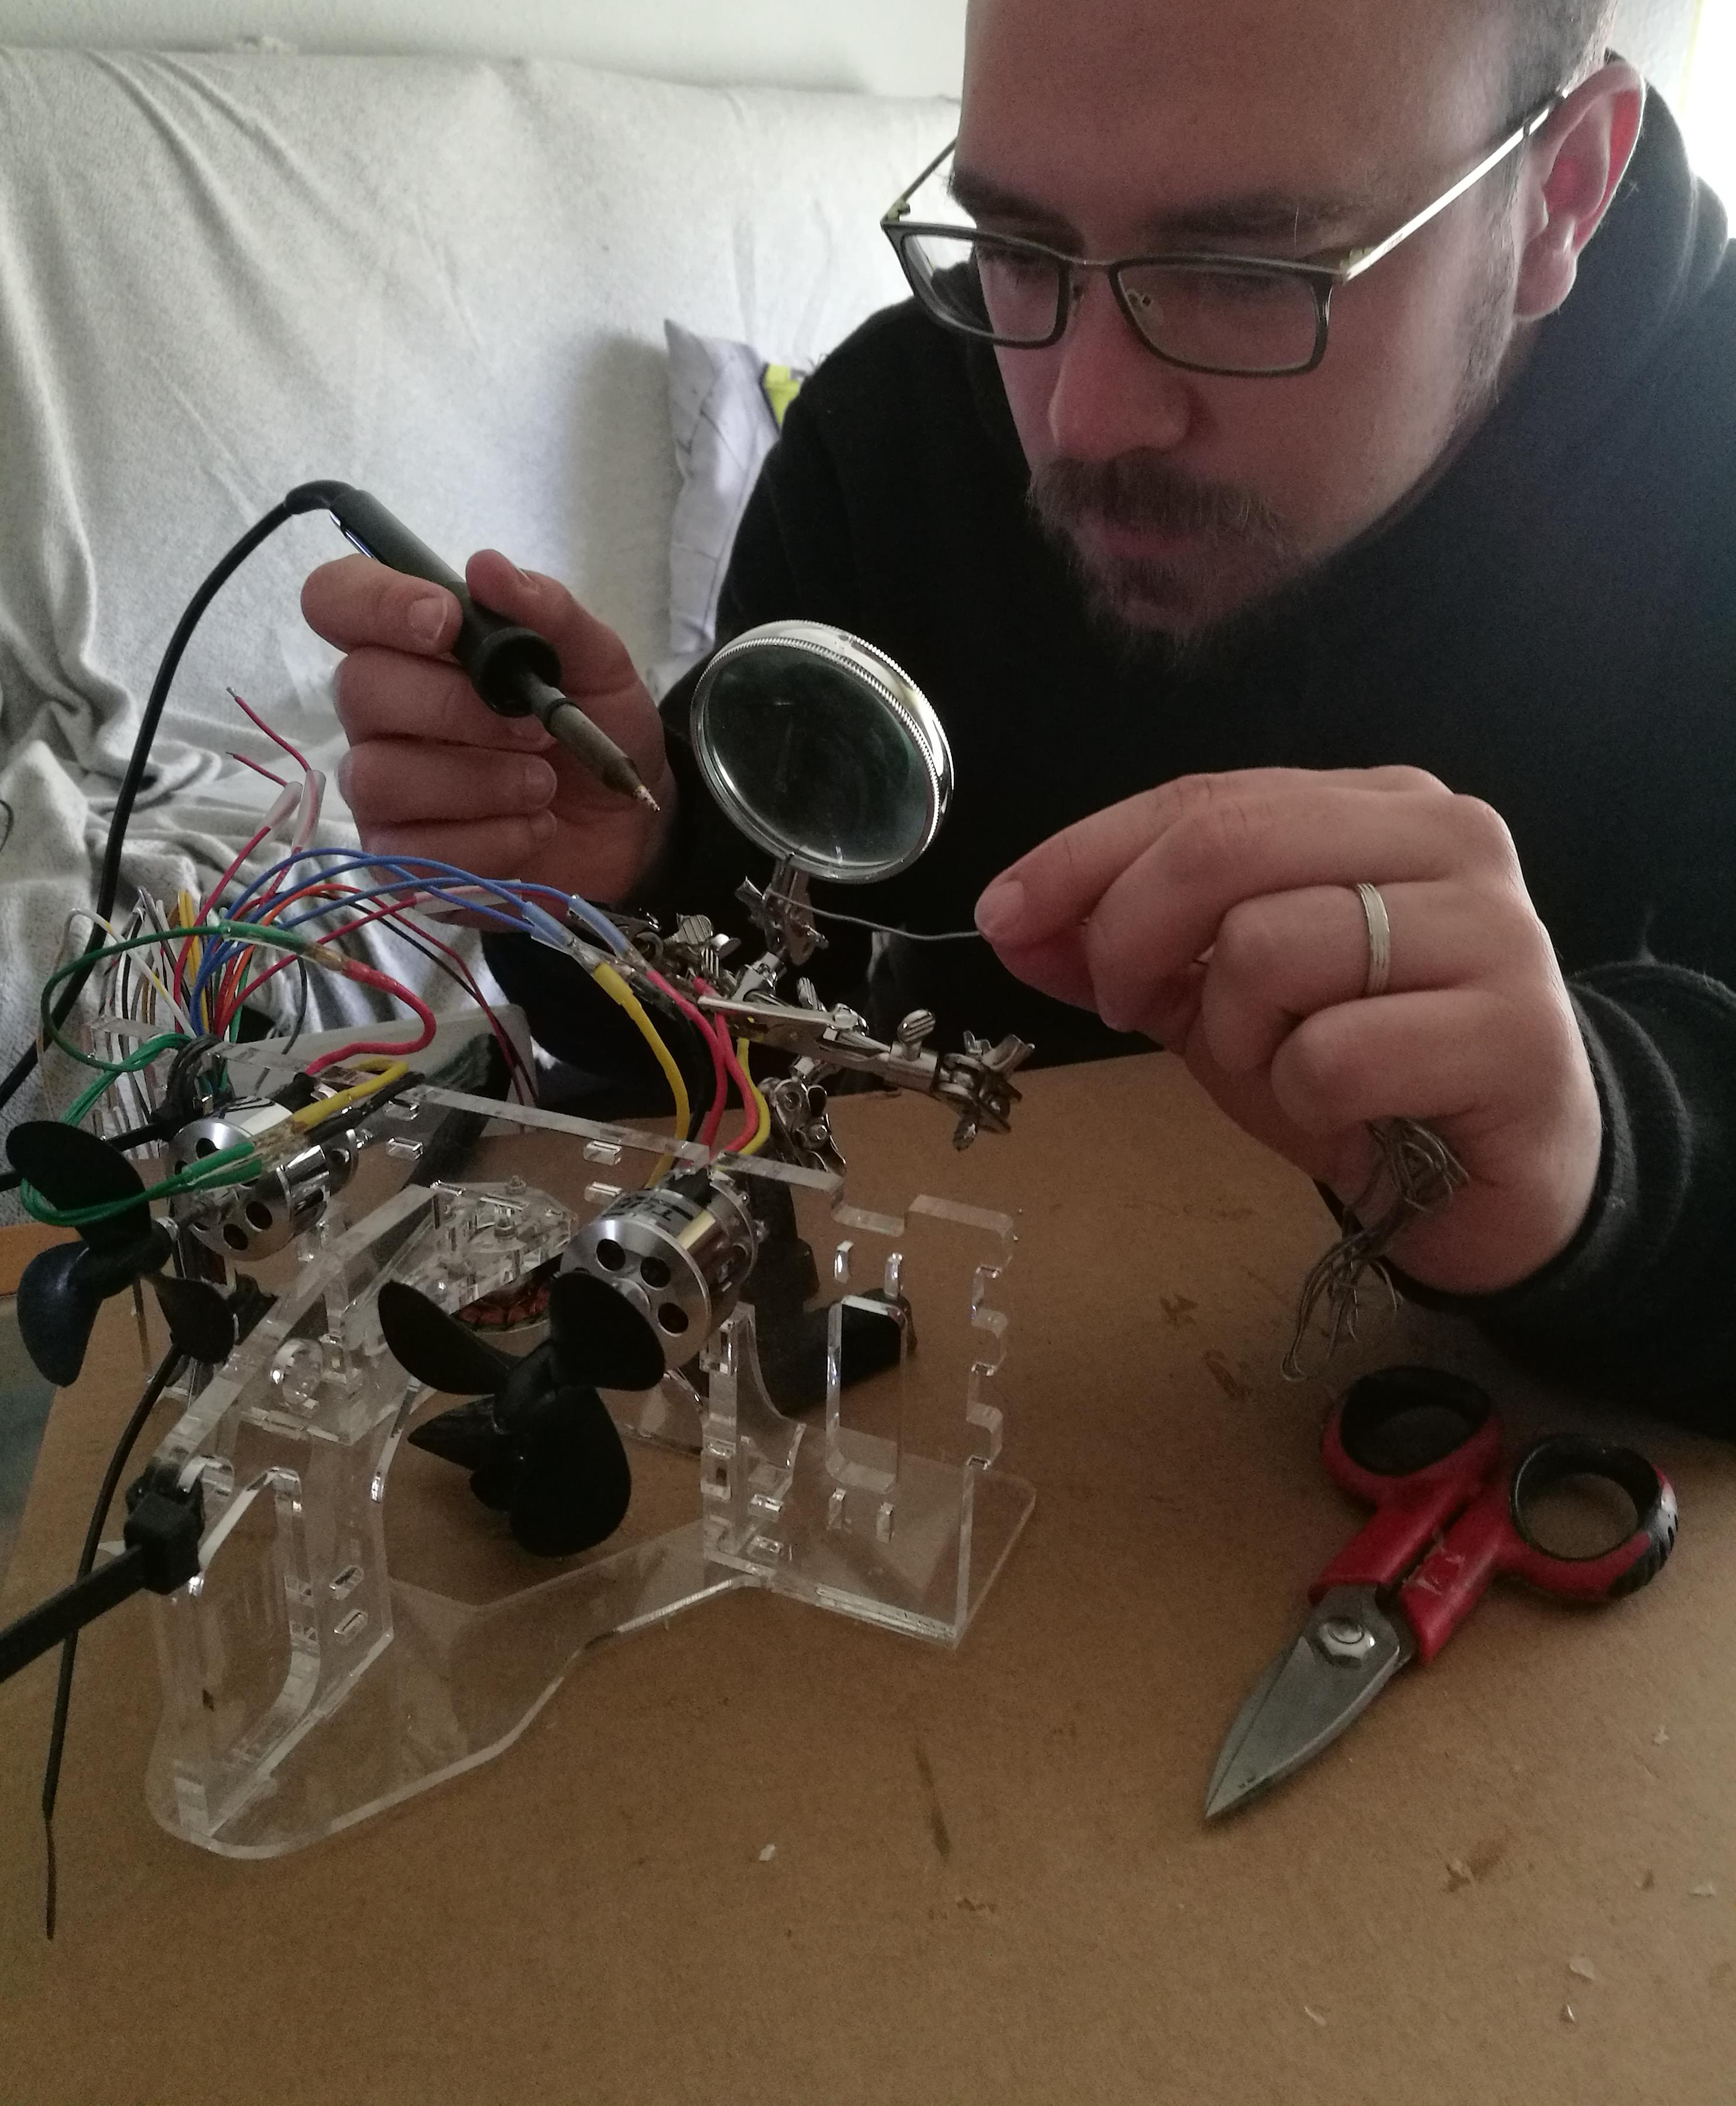
\includegraphics[width=5cm]{img/cap3/3_3/soldar}
  \end{center}
  \caption{Soldadura de cables}
  \label{fig:soldar}
\end{figure}

Los diez cables sobrantes se sellarán, ya que servirían para sensores y luces extra que no  utilizaremos en este proyecto.

Continuaremos con el montaje de los dos tubos de la batería. Primero, necesitaremos realizar el montaje de las piezas y soldaremos el muelle (borne) con un chip facilitado por la comunidad de ROV. Esta parte irá con el polo negativo de las baterías.
En el extremo del cable sobrante, se rellenará el terminal con estaño y se soldará al cable formando la parte positiva en la que se conectará la batería.

\subsection{Final}
\label{subsec:final}

En la parte final del montaje, será necesaria una soldadura con el cable de par trenzado que es el encargado de mandar la señal al portátil.

Para asegurar esa soldadura, utilizaremos una brida de un tamaño mayor a las usadas anteriormente, y soldaremos un cable preservado en el apartado anterior con el par trenzado.

Este cable de par trenzado mide cien metros, el cual, en el extremo opuesto al ROV, irá conectado al PLC. Gracias a este cable, el robot se podrá sumergir a una distancia de cien metros. Por eso, y para mayor seguridad, usaremos la brida, enroscaremos el cable en ella y lo finalizaremos recubriéndolo con cinta adhesiva.
En el cuerpo principal del ROV, sujetaremos con unas gomas los tubos que llevarán las baterías, y lo fijaremos en los extremos con dos varillas de metal.

Aislaremos el hardware con un tubo cilíndrico trasparente de polimetilmetacrilato, pero antes de fijarlo, limaremos los extremos del cilindro para una mejor conexión con las tapas.

Cuando todo el montaje esté terminado, pondremos más seguridad al hardware, añadiendo una cuerda que hará presión.

Además, colocaremos dos pesas de 300 gr. en los brazos del ROV para que la sumersión sea más fácil y fiable.

\section{Conectividad OpenROV}
\label{cap:Conectividad OpenROV}
  
En esta sección se marcarán las pautas necesarias para realizar el correcto funcionamiento del software del OpenROV.  
  
\subsection{Diseño de Conectividad}
\label{subsec:disenio}

Para encender el ROV, necesitaremos el cable mini USB y el cable ethernet debidamente colocado en el extremo del PLC y estos a su vez al portátil.

\begin{figure} [hbtp]
\begin{center}
  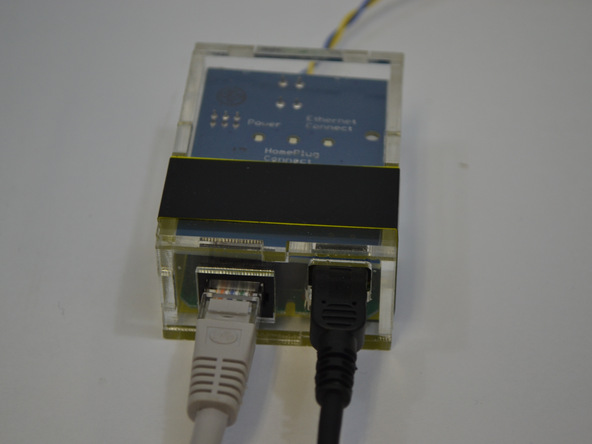
\includegraphics[width=8cm]{img/cap3/3_4/plc_externo}
\end{center}
\caption{PLC externo}
\label{fig:plc_ext}
\end{figure}
  
El conector USB actúa como interruptor de encendido/apagado del robot.

El ROV tiene una dirección IP estática 192.168.254.1. Para conectarnos a la web del robot, la dirección ethernet de nuestro ordenador debe pertenecer a la misma subred, es decir, 192.168.254.2. La máscara de subred se establece en la dirección 255.255.255.0.

Pero para poder mostrar la página, antes debemos realizar una serie de pasos, en la que necesitaremos una tarjeta microSD para realizar la configuración del ROV.
  
\begin{enumerate}
\item Se descarga la imagen más reciente de OpenROV 2.8, en este caso, la versión es 30.0.3. Una vez descargado, se descomprime el archivo .zip, dejando en el directorio de descarga un ficherom con la extensión .img.
\item Formateamos la tarjeta microSD, y montaremos la imagen descargada en la tarjeta. Una vez terminado el proceso, quitaremos la tarjeta del portátil.
\item Conectamos la tarjeta microSD a el Beagle Bone, y conectamos el ROV con el cable USB para encenderlo. Los LED de la placa Beagle Bone parpadearán para mostrar que la imagen se está aplicando a la memoria de la placa. El proceso termina cuando los cuatro led se queden encendidos, si pasado un tiempo los cuatro leds no lucen, habría que repetir este punto.

Cuando esté completo, retiraremos el cable USB del portátil para desconectar el ROV y retiraremos la tarjeta microSD de la placa Beagle Bone.

Terminado este proceso, volveremos a conectar la tarjeta en el portátil.
\newpage
\begin{figure} [hbtp]
\begin{center}
  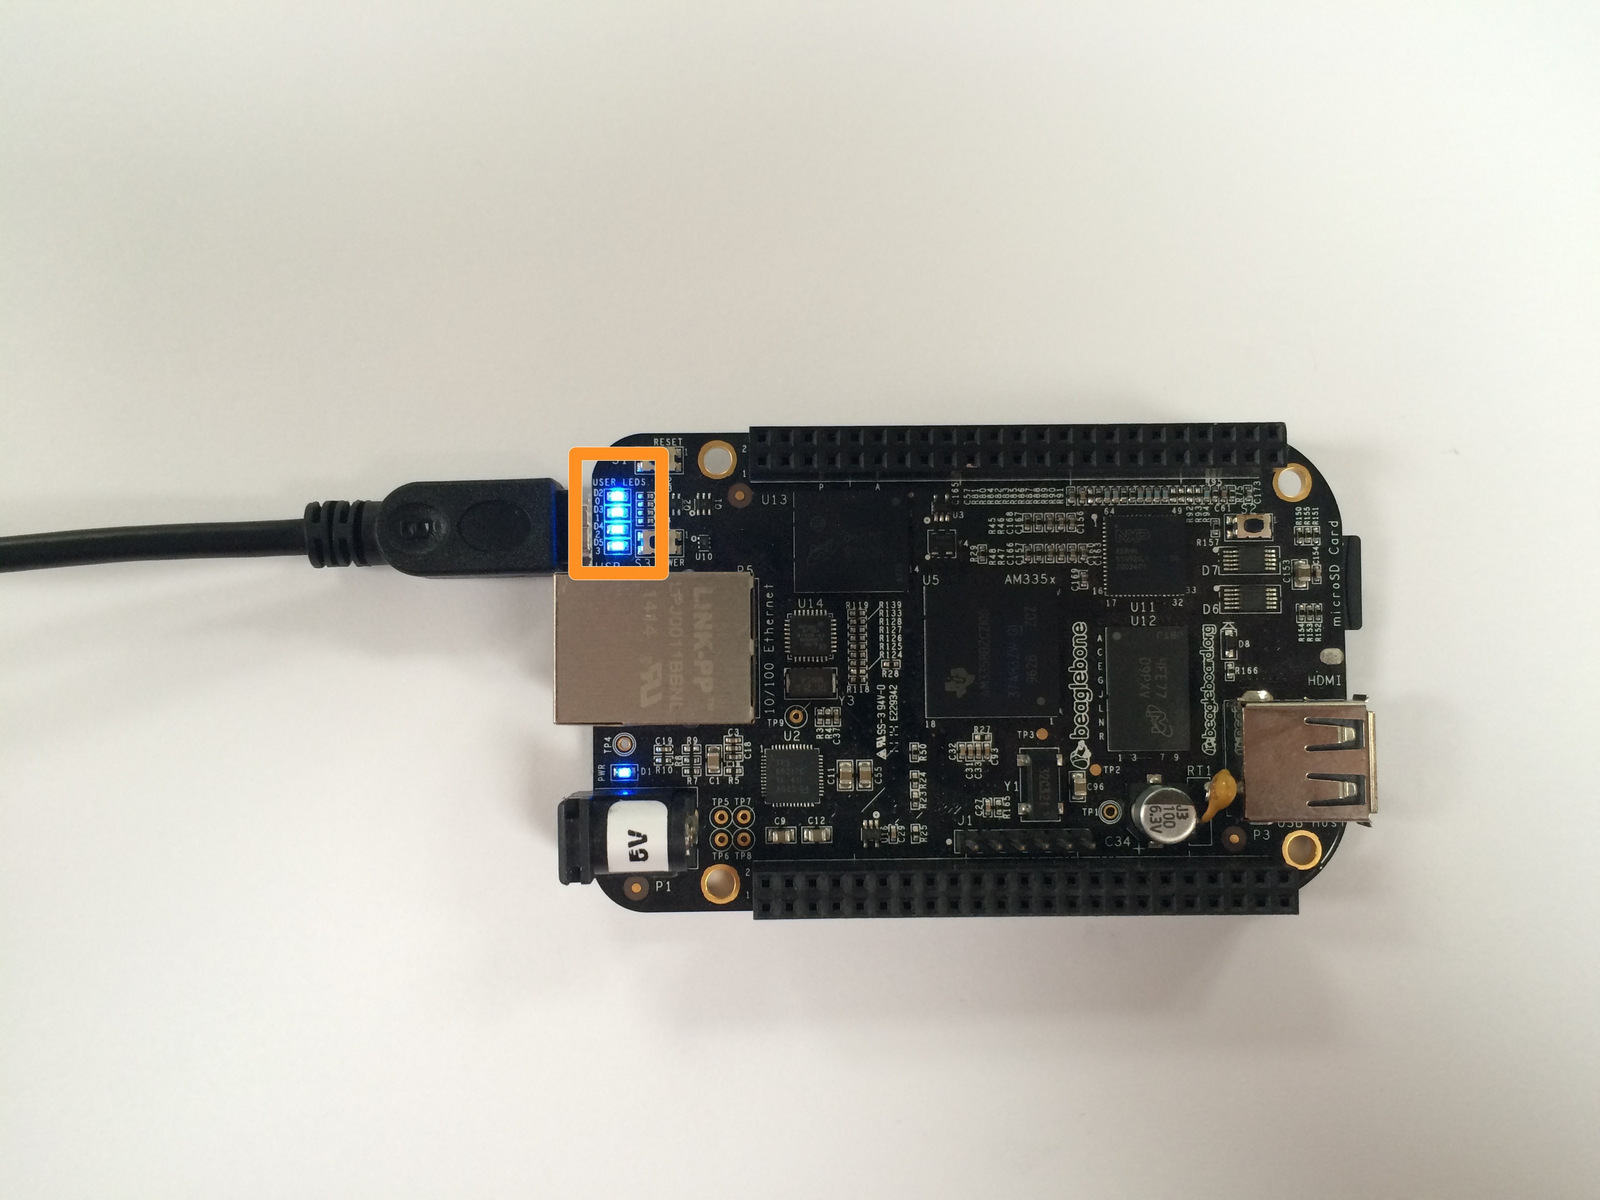
\includegraphics[width=8cm]{img/cap3/3_4/BBB}
\end{center}
\caption{BeagleBone configurada}
\label{fig:bbb}
\end{figure}
\item Como se mencionó al principio del apartado, el ROV tiene una dirección IP estática incorporada de 192.168.254.1. Para conectarnos, configuraremos nuestro ordenador con la dirección IP 192.168.254.2 y con la máscara de subred en la dirección 255.255.255.0.

En Windows 8 la configuración sería:

\renewcommand{\lstlistingname}{Configuración}
\begin{lstlisting}[caption= Windows 8, label={lst:config_w8}]
Ir  al Panel de control.
Seleccionar Red e Internet.
Red y centro compartido → (click) cambiar configuración de adaptador → (click) ethernet.
Propiedades →(click) usar la siguiente dirección IP
Insertarla dirección IP 192.168.254.2
\end{lstlisting}

\begin{figure} [hbtp]
\begin{center}
  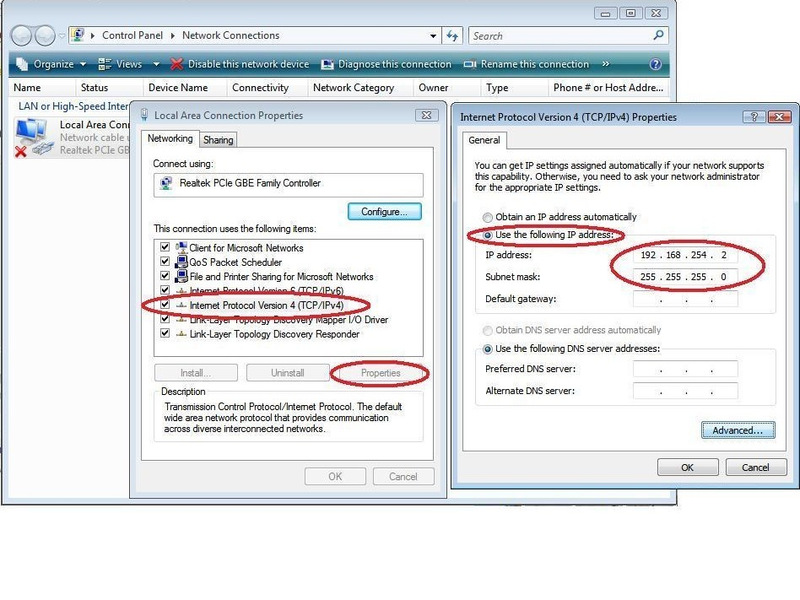
\includegraphics[width=6cm]{img/cap3/3_4/conexion}
\end{center}
\caption{Conexión Windows 8}
\label{fig:w8}
\end{figure}
\newpage
En Ubuntu la configuración de una nueva IP estática:

\renewcommand{\lstlistingname}{Configuración}
\begin{lstlisting}[caption= Ubuntu, label={lst:config_ubuntu}]
  # Abrir el terminal (Ctrl + Atl + T).
  # Comprobamos las interfaces del equipo:  
  $ ifconfig -a
  # Editamos el archivo de configuracion de las interfaces:  
  $ sudo vim /etc/network/interfaces

  # Configuracion de direccion IP fija para el interfaz eth0
    auto eth0
    iface eth0 inet static
    address 192.168.254.2
    netmask 255.255.255.0
    network 192.168.254.0
    broadcast 192.168.254.255
    gateway 192.168.254.1
\end{lstlisting}

  Donde:
    \subsubitem address es la dirección IP que quieres ponerle a tu máquina.
    \subsubitem netmask es la máscara de subred de esa dirección IP.
    \subsubitem network es la red a la que pertenece esa dirección IP.
    \subsubitem broadcast es la direción IP de difusión de esa red.
    \subsubitem gateway es la dirección IP de la puerta de enlace predeterminada.

\subitem Reiniciamos las interfaces de red para aplicar los cambios:

\renewcommand{\lstlistingname}{}
\begin{lstlisting}[caption=Reinicio, label={lst:reset}]
  $ sudo /etc/init.d/networking restart
\end{lstlisting}
\item Abriremos el navegador Google-Chrome, y en la barra de direcciones escribiremos la IP 192.168.254.1:8080, que es la dirección IP de OpenROV. Accederemos a la web, que es la interfaz de OpenROV.
\item Para finalizar, deberemos actualizar el firmware, en la web, presionaremos el botón de configuración en la parte superior derecha de la pantalla y presionaremos “Cargar firmware desde la tarjeta SD a Ardruino”
La tarjeta microSD no debe estar en el ROV, presionaremos “Mostrar Detalles” y seguidamente, “Aplicar nuevo Firmware”.
Una vez que la carga sea exitosa, como el de la imagen, se retirará el cable USB del portátil para desconectar el ROV. Volveremos a conectar el cable USB al portátil para realizar el reinicio.


\begin{figure} [hbtp]
\begin{center}
  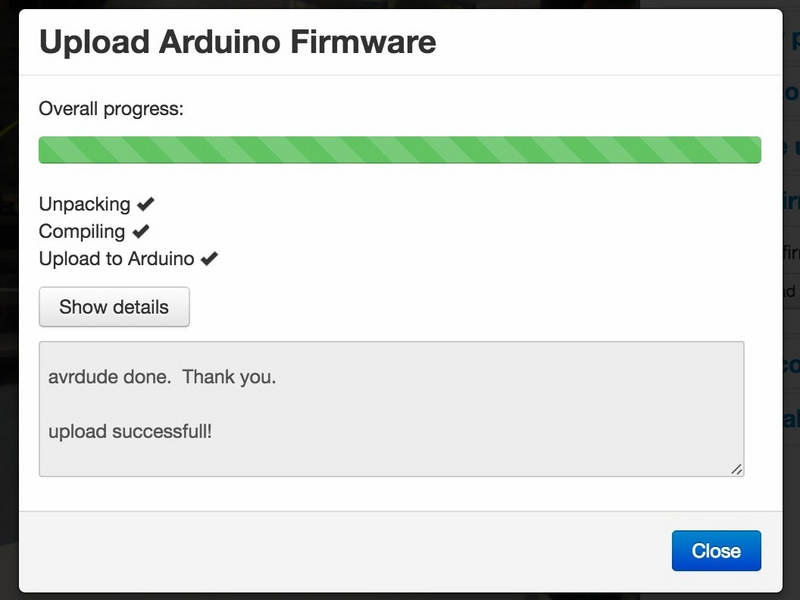
\includegraphics[width=8cm]{img/cap3/3_4/firmware}
\end{center}
\caption{Actualización firmware}
\label{fig:firmware}
\end{figure}

\end{enumerate}
  
  
  
\subsection{Puesta a punto de los elementos}
\label{subsec:elementos}
  \subsubsection{Cámara}
  \label{subsubsec:camara}
Ajustaremos el foco de la lente de la cámara hasta que la imagen pueda verse con nitidez.
\begin{figure} [hbtp]
\begin{center}
  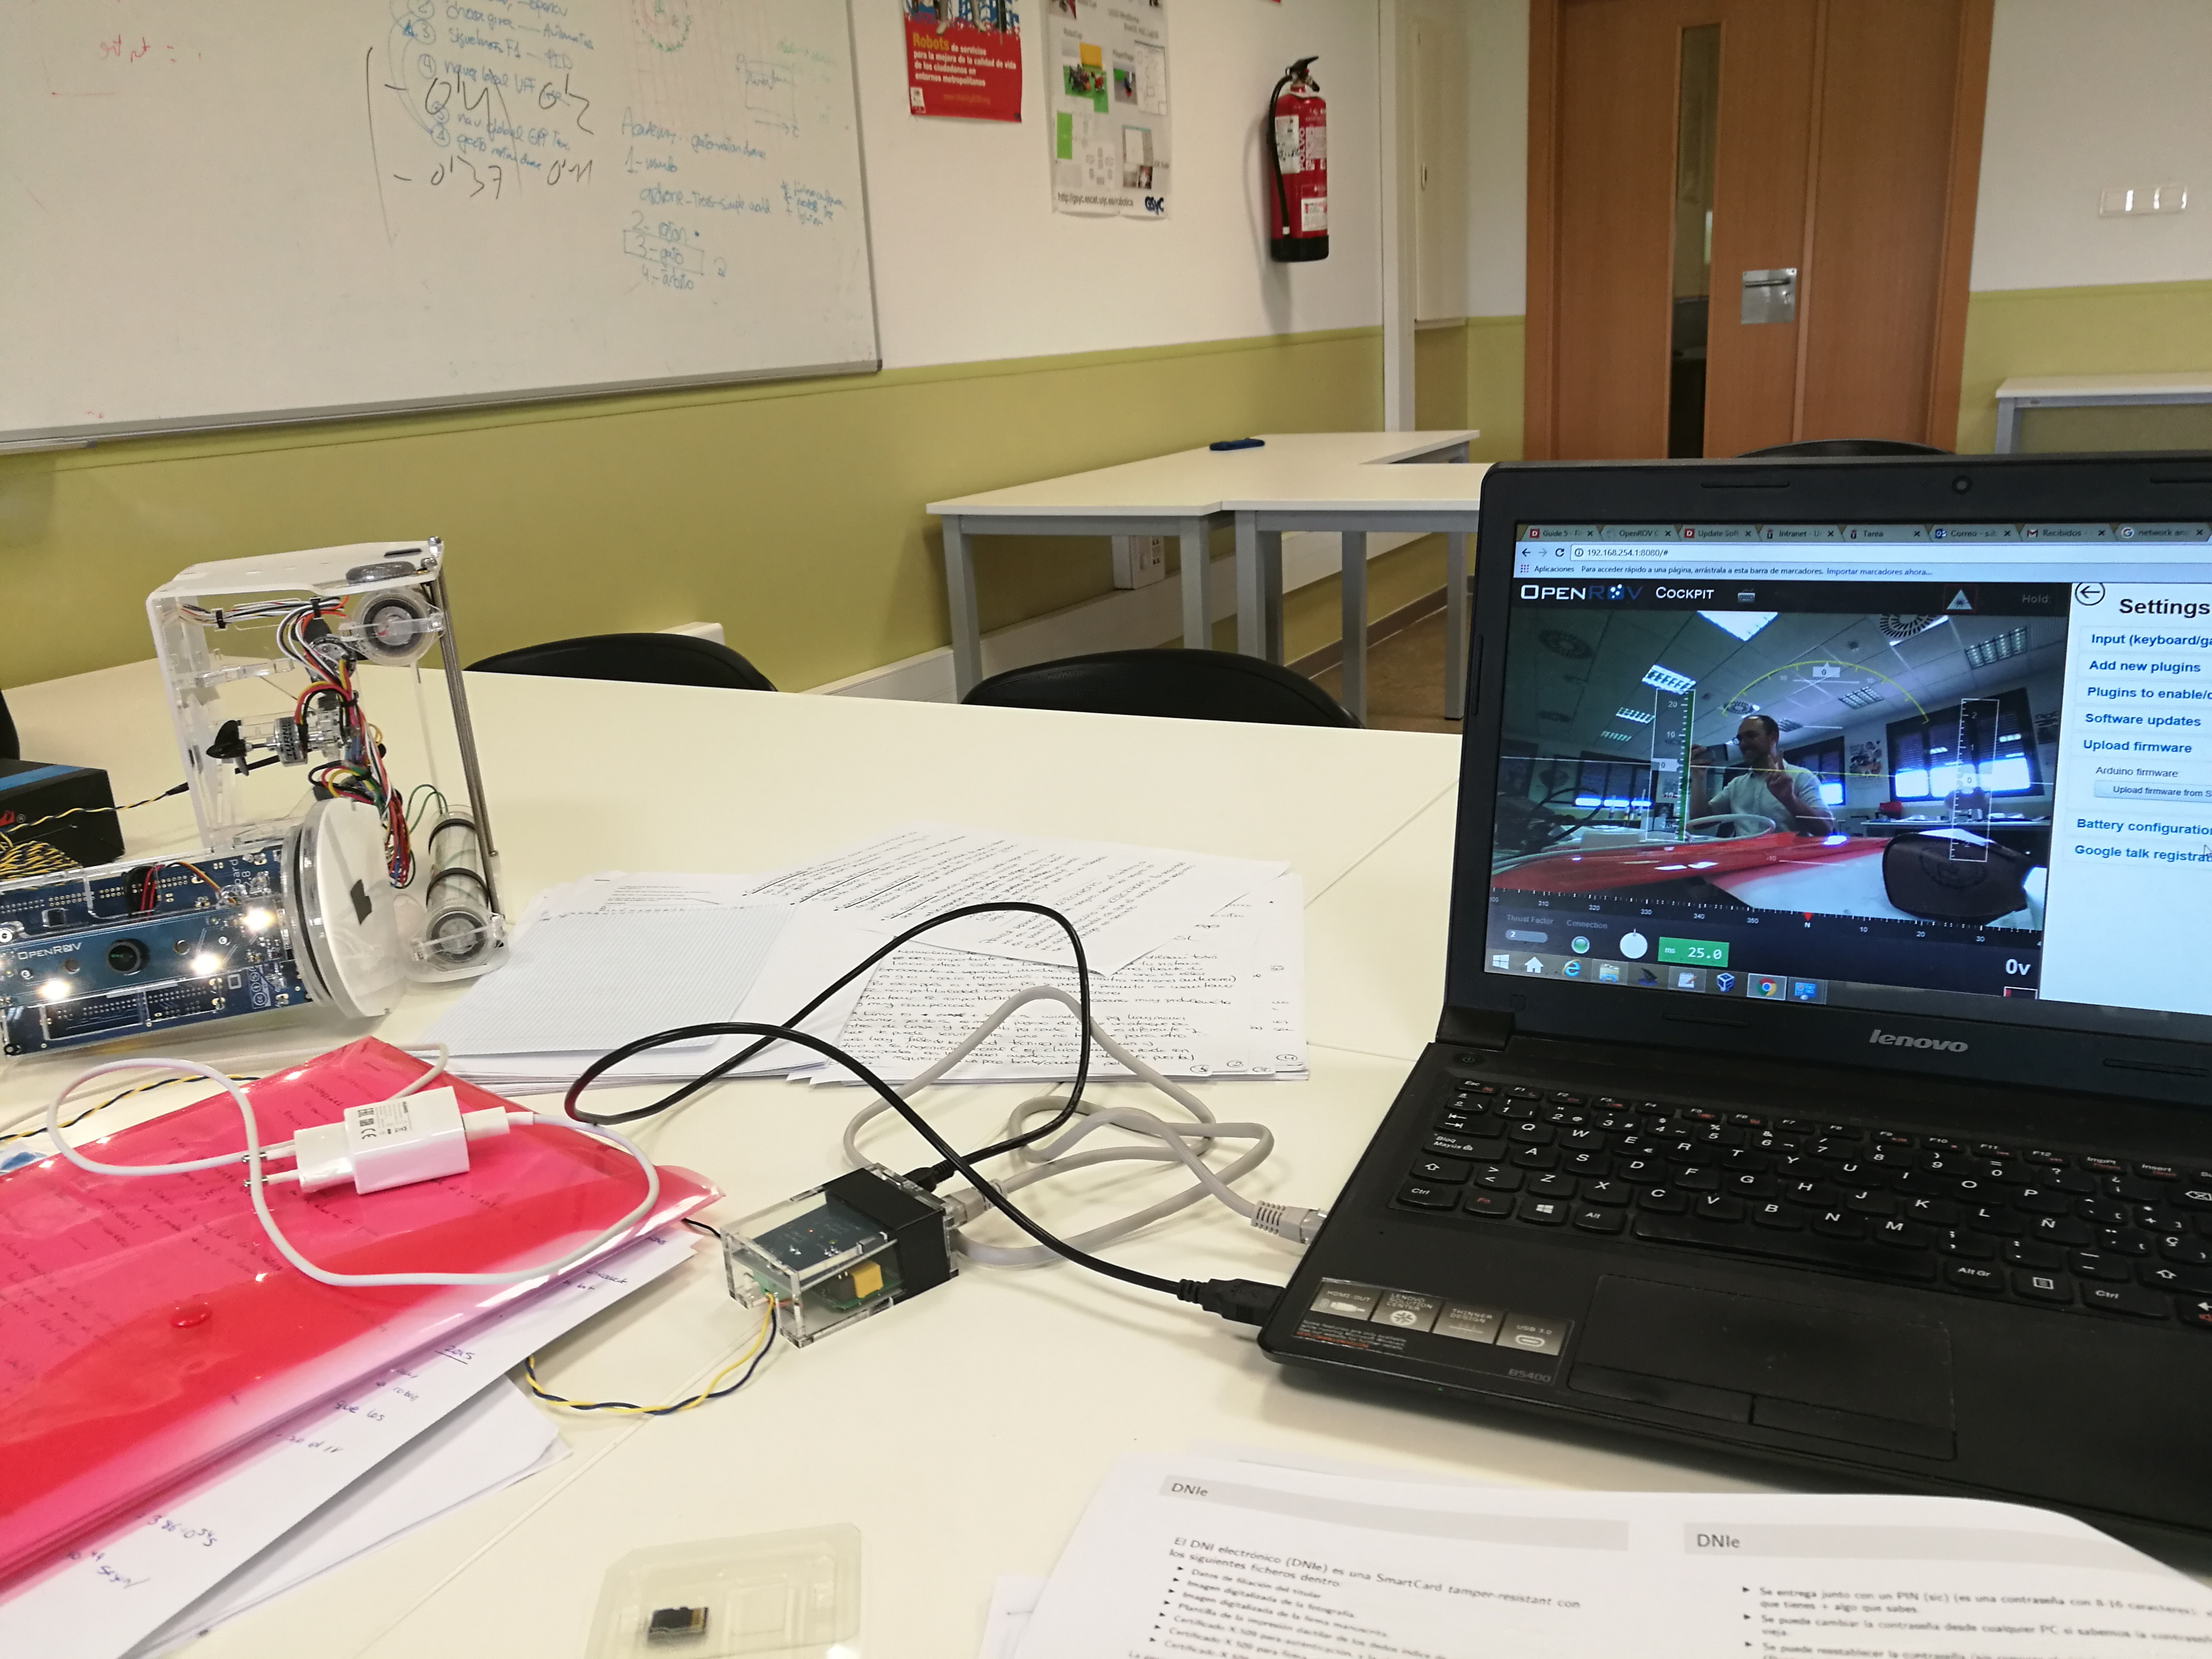
\includegraphics[width=8cm]{img/cap3/3_4/foco}
\end{center}
\caption{Foco cámara}
\label{fig:foco}
\end{figure}
    
  \subsubsection{Láser}
  \label{subsubsec:laser}
El ROV lleva incorporado dos láser, que hemos soldado previamente a la placa de la cámara. El proceso que llevaremos a cabo será su calibración y pegado en el chásis.
En un papel dibujaremos dos “X” separadas entre si diez centímetros, y colocaremos esa hoja a una distancia de entre tres y cuatro metros del robot, el cual, debe estar a la misma altura que el folio.
Si pesionamos la tecla L en la web, encenderemos los láseres. Para apagarlos, simplemente hay que volver a pulsar la tecla L.
Una vez este todo calibrado, pegaremos con Super Glue los láseres al chasis de la cámara.
 \begin{figure}[hbtp]
  \begin{center}
    \subfigure[Distancia de los laseres]{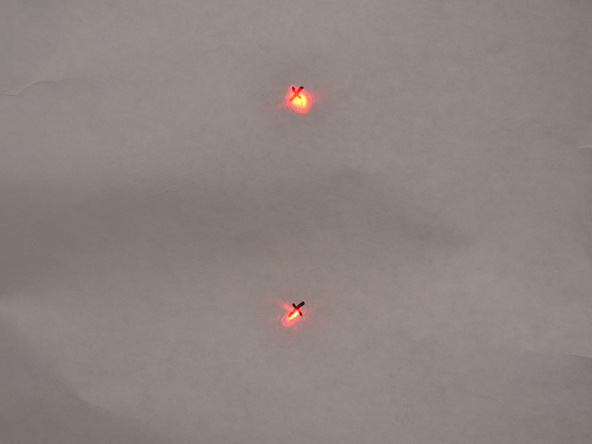
\includegraphics[width=6cm,height=5cm]{img/cap3/3_4/laseres}}
    \subfigure[Fijado del los laseres]{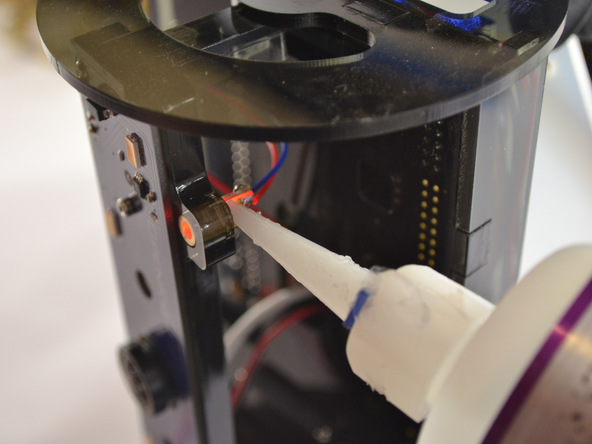
\includegraphics[width=6cm,height=5cm]{img/cap3/3_4/laser_camara}}
  \end{center}
  \caption{Láser}
  \label{fig:laser}
\end{figure}
  
\subsubsection{Motores}
\label{subsubsec:motores}
En este punto, se realizará una comprobación de las hélices. Para ver si su rotación es la correcta presionaremos la tecla de “flecha arriba”, y observaremos en que dirección giran los motores.
El motor izquierdo (amarillo) debe funcionar en sentido contrario a las agujas del reloj.
El motor derecho (azul) debe funcionar en sentido a las agujas del reloj.
\begin{figure} [hbtp]
\begin{center}
  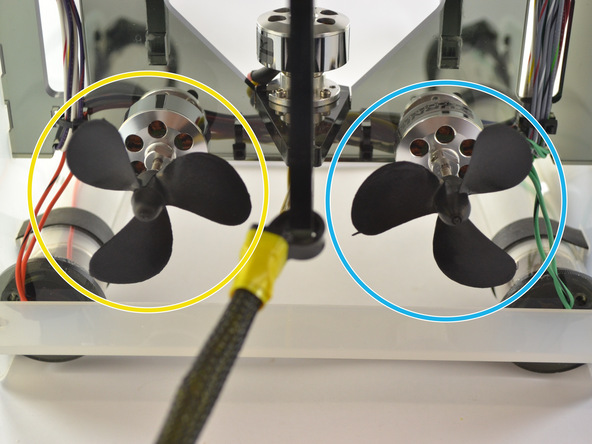
\includegraphics[width=8cm]{img/cap3/3_4/motores}
\end{center}
\caption{Motores}
\label{fig:motores}
\end{figure}

Si el giro es incorrecto, invertiremos su rotación en la parte de “diagnóstico” de la web. Seleccionaremos la opción “invertir” del motor o motores que queramos modificar.

\begin{figure} [hbtp]
\begin{center}
  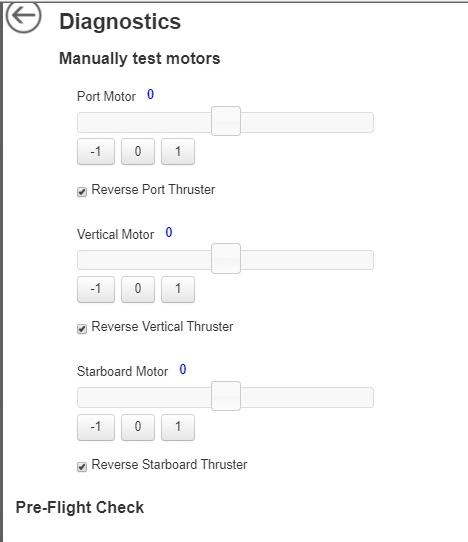
\includegraphics[width=7cm]{img/cap3/3_4/diagnostic}
\end{center}
\caption{Diagnostics}
\label{fig:diagnostics}
\end{figure} 

\subsubsection{Tubo cilíndrico trasparente de polimetilmetacrilato}
\label{subsubsec:tubo}
El tubo cilíndrico contendrá todo el sistema hardware y software del ROV.
Para una mejor fijación, lijaremos los bordes interiores para que la junta se ajuste al tubo.
\begin{figure} [hbtp]
\begin{center}
  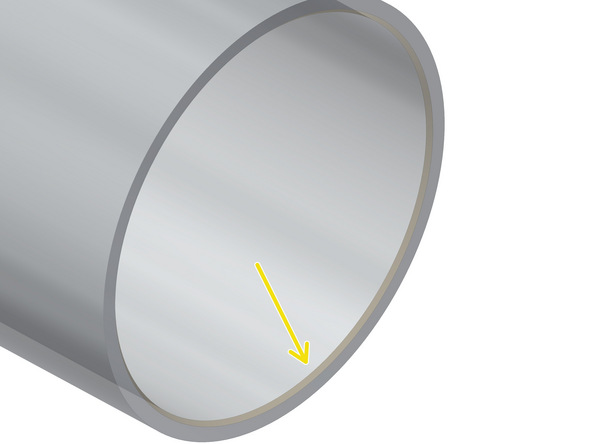
\includegraphics[width=8cm]{img/cap3/3_4/tubo}
\end{center}
\caption{Tubo}
\label{fig:tubo}
\end{figure}

\subsubsection{Tapa superior}
\label{subsubsec:tapa}
Una vez instalado el tubo, verificamos de que la junta esté bien introducida a lo largo de todo el perímetro interior del tubo.
La tapa superior contiene un orificio de ventilación para igualar la presión al colocar las tapas.
\begin{figure} [hbtp]
\begin{center}
  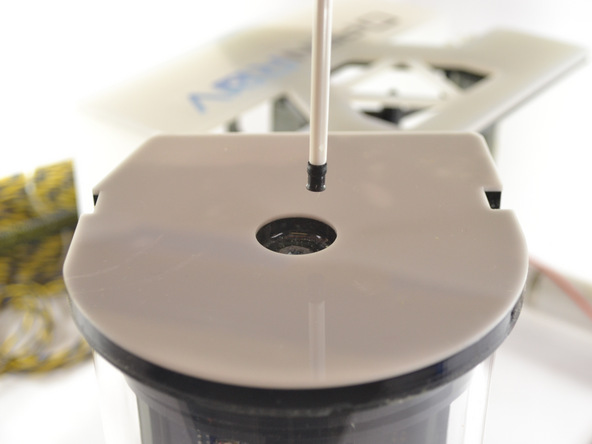
\includegraphics[width=8cm]{img/cap3/3_4/tapa_superior}
\end{center}
\caption{Tapa superior}
\label{fig:tapa_sup}
\end{figure}  

\newpage
\subsection{Web/Cockpit}
\label{subsec:cockpit}
El manejo del ROV se consigue gracias a la web Cockpit, que es la interfaz de usuario y contiene todos los sistemas de control de cualquier vehículo o dispositivo operado a distancia.

\begin{figure} [hbtp]
\begin{center}
  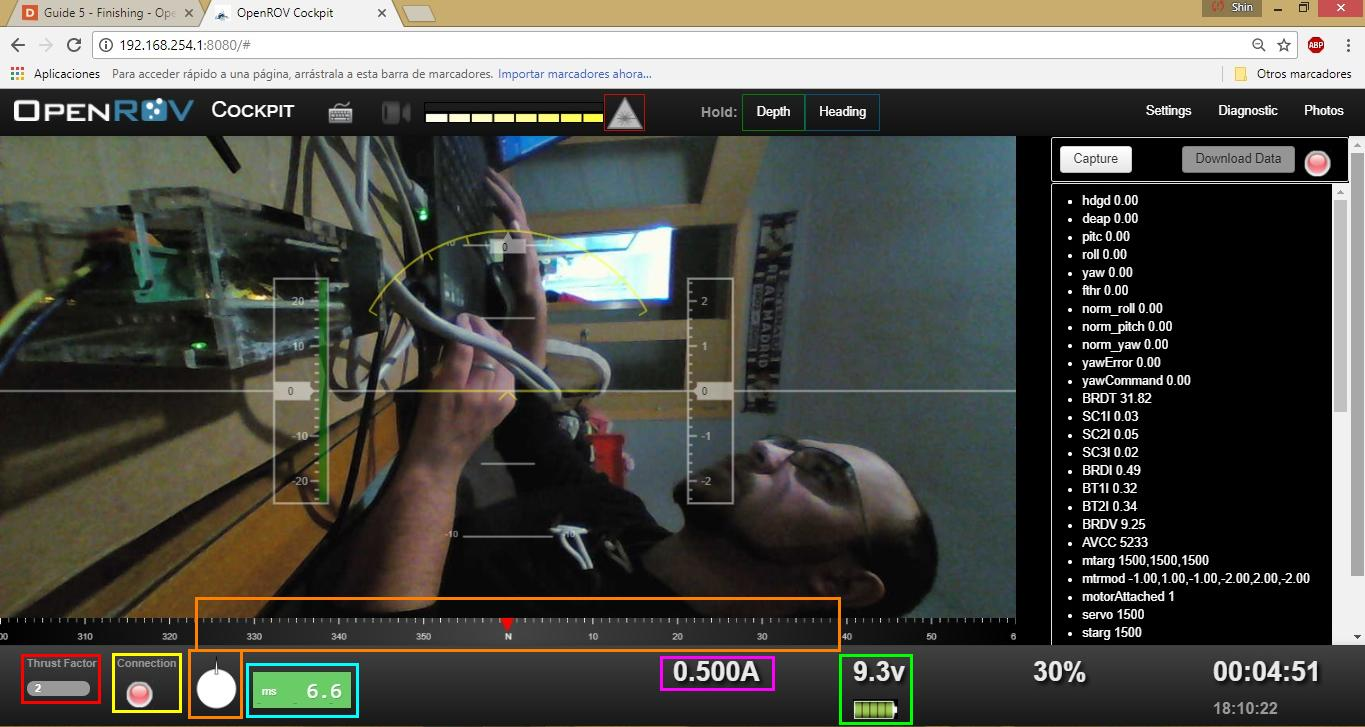
\includegraphics[width=15cm]{img/cap3/3_5/cockpit1_v2}
\end{center}
\caption{Cockpit (1)}
\label{fig:cockpit1}
\end{figure}

\begin{itemize}
\item[\textcolor{red}{\textbullet}]Configuración de potencia de los motores (1, la más baja y 5, la más alta).
\item[\textcolor{yellow}{\textbullet}]Conectividad (verde = conectado).
\item[\textcolor{orange}{\textbullet}]Brújula.
\item[\textcolor{blue}{\textbullet}]Latencia (si hubiera algún problema mostraría +999).
\item[\textcolor{purple}{\textbullet}]Intensidad de corriente los componentes electrónicos en Amperios.
\item[\textcolor{green}{\textbullet}]Potencia de las baterías.
\end{itemize}

\begin{figure} [hbtp]
\begin{center}
  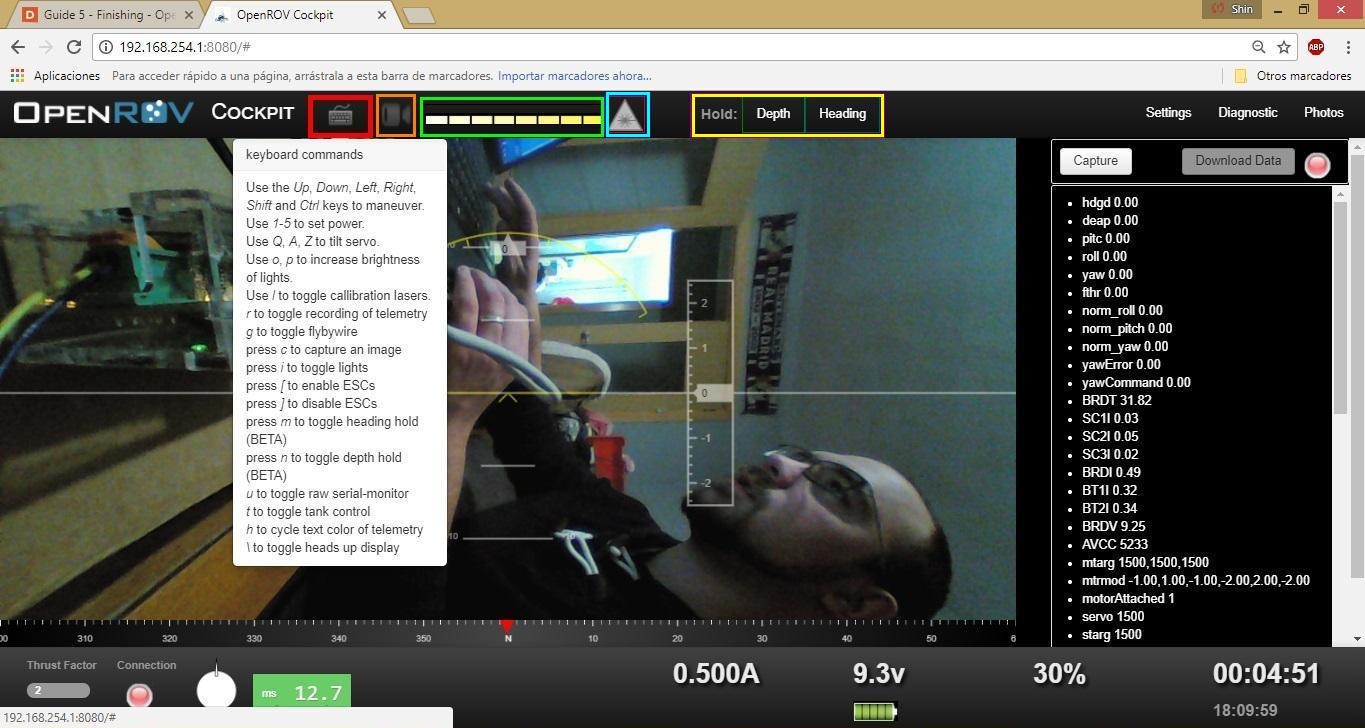
\includegraphics[width=15cm]{img/cap3/3_5/cockpit2_v2}
\end{center}
\caption{Cockpit (2)}
\label{fig:cockpit2}
\end{figure}

\begin{itemize}
\item[\textcolor{red}{\textbullet}]Pulsando el botón señalado en rojo (el icono del teclado) se obtienen los comandos de uso del robot.
\item[\textcolor{orange}{\textbullet}]Indicador de la cámara.
\item[\textcolor{green}{\textbullet}]Indicador de nivel de luz.
\item[\textcolor{blue}{\textbullet}]Indicador de encendido/apagado del láser.
\item[\textcolor{yellow}{\textbullet}]Indicadores de profundidad y rumbo. Se alternan entre activo/desactivo para mantener la profundidad actual y/o el rumbo.
\end{itemize}


\newpage
\begin{figure} [hbtp]
\begin{center}
  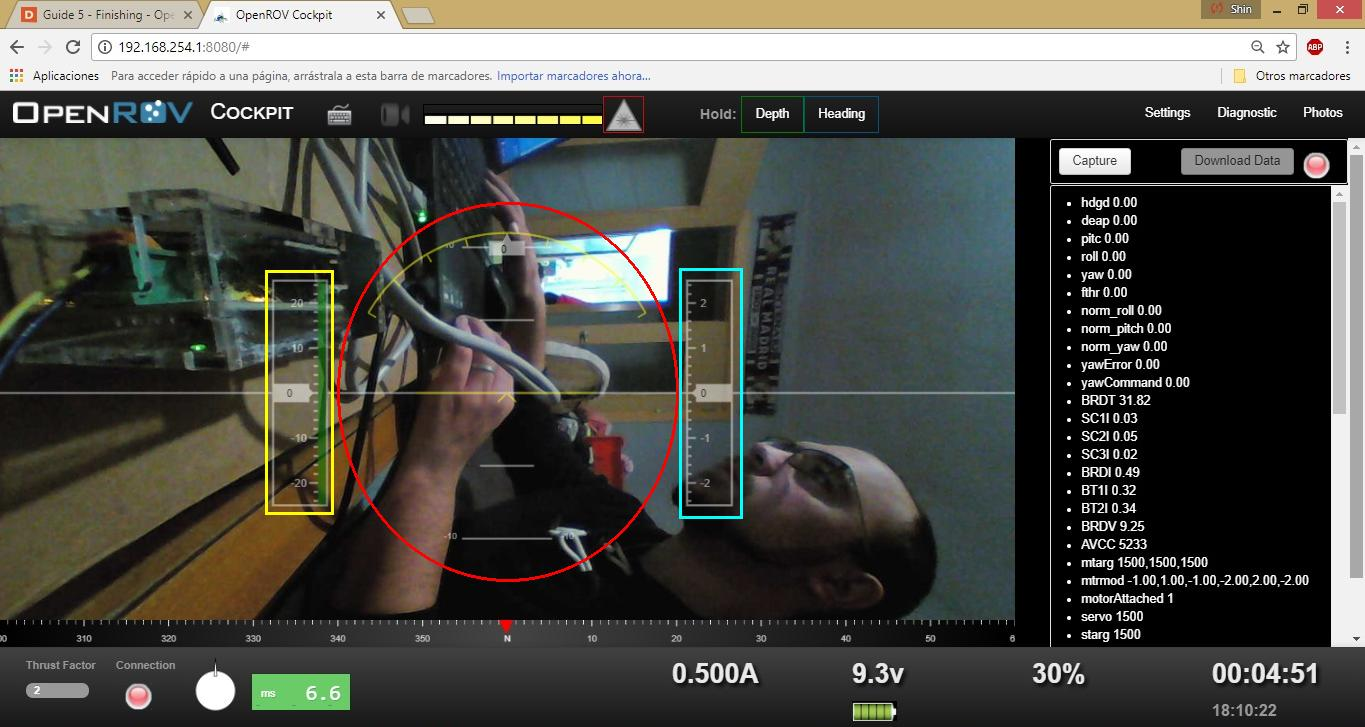
\includegraphics[width=15cm]{img/cap3/3_5/cockpit3_v2}
\end{center}
\caption{Cockpit (3)}
\label{fig:cockpit3}
\end{figure}
\begin{itemize}
\item[\textcolor{yellow}{\textbullet}]Fuerza de empuje del motor.
\item[\textcolor{red}{\textbullet}]Horizonte artificial.
\item[\textcolor{green}{\textbullet}]Profundidad.
\end{itemize}

\begin{figure} [hbtp]
\begin{center}
  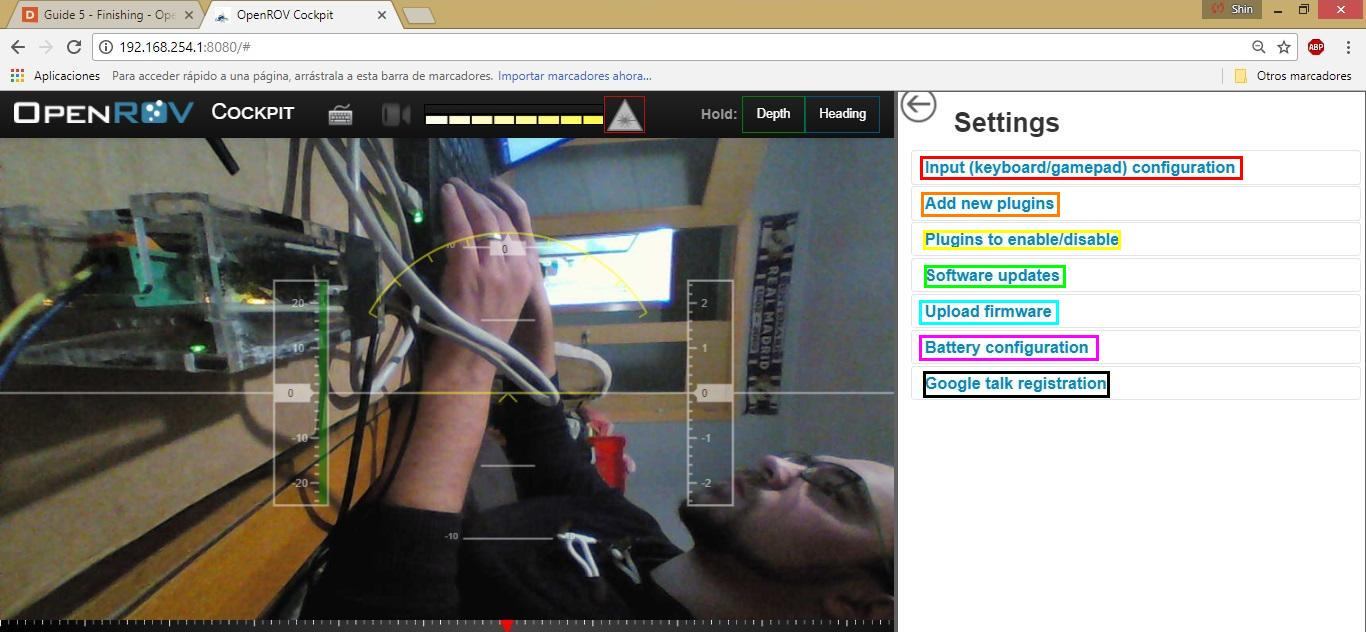
\includegraphics[width=15cm]{img/cap3/3_5/setting}
\end{center}
\caption{Ajustes}
\label{fig:settting}
\end{figure}
\newpage
Panel de configuración:
\begin{itemize}
 \item[\textcolor{red}{\textbullet}] Configuración de entrada: personalizar las comandos de uso del robot.
 \item[\textcolor{orange}{\textbullet}] Agregar nuevos complementos.
 \item[\textcolor{yellow}{\textbullet}] Habilitar/deshabilitar complementos: activa y desactiva los complementos agregados en el punto anterior.
 \item[\textcolor{green}{\textbullet}] Actualización de software.
 \item[\textcolor{blue}{\textbullet}] Actualización del firmware.
 \item[\textcolor{purple}{\textbullet}] Configuración de la batería: Se establece el voltaje mínimo y máximo de la batería.
 \item[\textcolor{black}{\textbullet}] Registro de Google Talk: Permite el acceso a las de redes sociales de la web.
 \end{itemize}

\begin{figure} [hbtp]
\begin{center}
  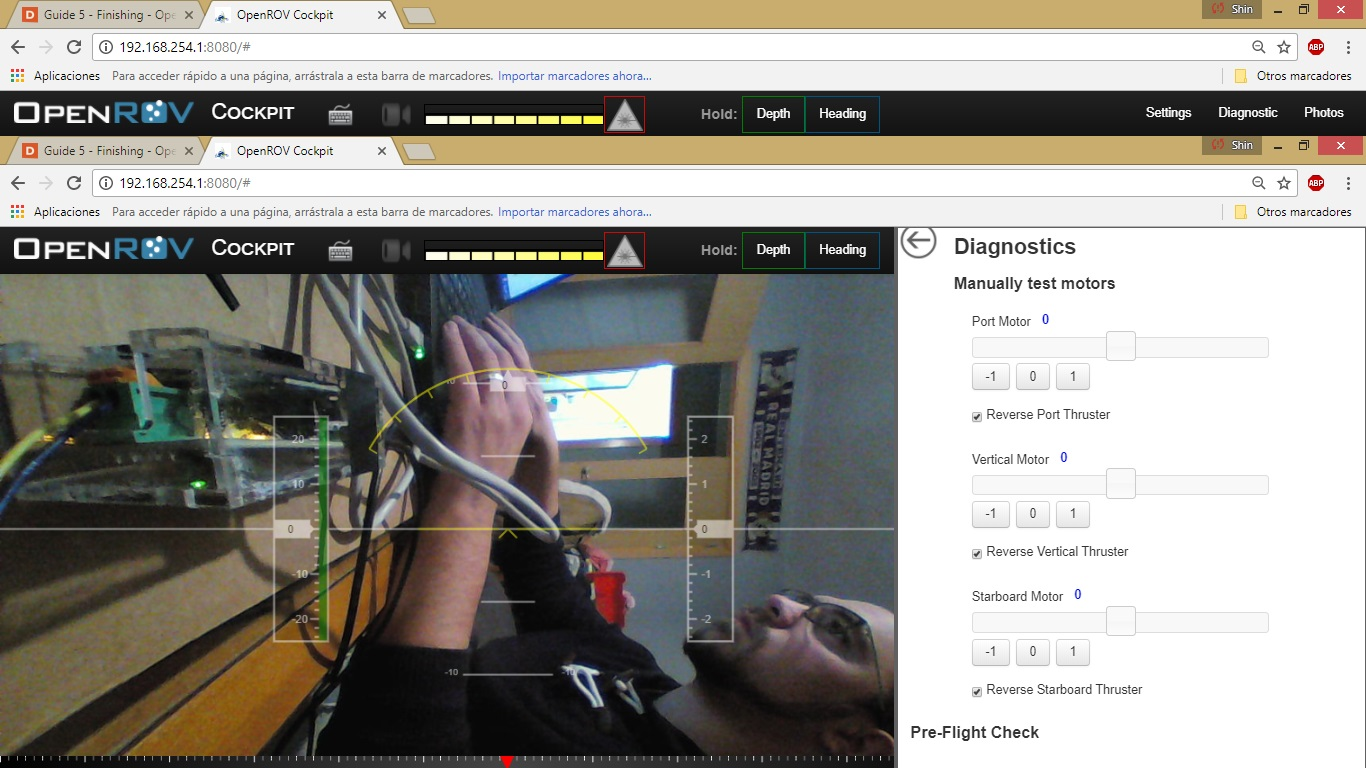
\includegraphics[width=15cm]{img/cap3/3_5/diagnostico}
\end{center}
\caption{Diagnóstico}
\label{fig:diagnostico}
\end{figure}

Panel de diagnósticos:
\begin{itemize}
 \item Verificación manual los motores.
 \item Si hay un error con la dirección de los motores se puede invertir desde este panel.
 \item Pre-Flight Check, es el marcador de la posición actual.
\end{itemize}

\begin{figure} [hbtp]
\begin{center}
  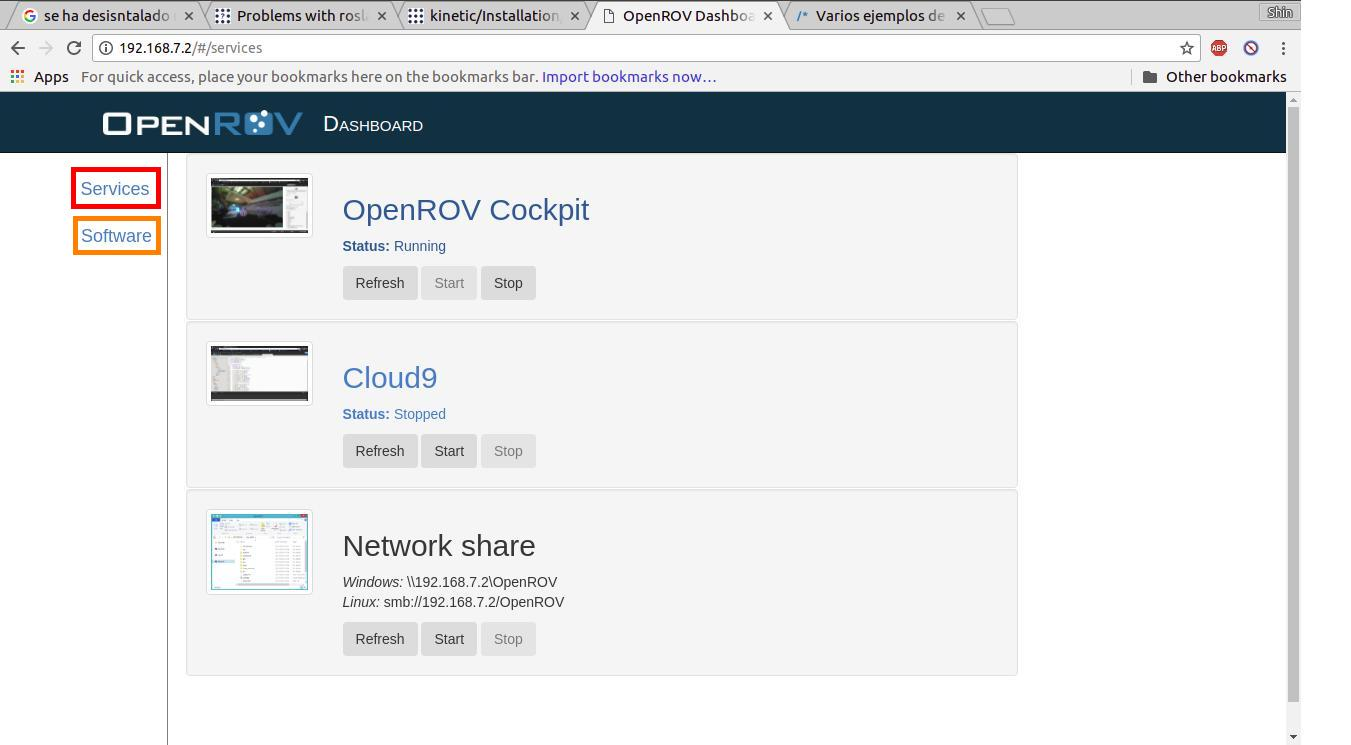
\includegraphics[width=15cm]{img/cap3/3_5/services}
\end{center}
\caption{Servicios}
\label{fig:services}
\end{figure}

El panel de configuración de OpenROV se encuentra en: 192.168.254.1

Hay dos partes:
\begin{itemize}
\item[\textcolor{red}{\textbullet}]\textbf{Servicios}: Reiniciar la web del ROV.
\item[\textcolor{orange}{\textbullet}]\textbf{Software}: Determinar la versión del software y puede ejecutar la actualización del software del ROV.
\end{itemize}

\subsection{Mantenimiento}
\label{subsec:mantenimiento}

Para que la vida útil del robot sea lo más larga posible, se deben seguir unas ciertas pautas de mantenimiento.

\subsubsection{Enjuagar}
\label{subsubsec:enjuagar}
Una vez que hayamos utilizado el robot, tendremos que enjuagarlo en agua después de cada inmersión, para mantenerlo limpio y libre de desechos y minerales.
  
\subsubsection{Mantenimiento de los motores}
\label{subsubsec:mantenimiento}
Después de haber utilizado el robot en una inmersión, se debe limpiar los motores, ya que tienden a corroerse fácilmente. Se recomienda lubricarlos.
Los pasos que debemos seguir son los siguientes:
\begin{enumerate}
\item Enjuagar los motores en agua fría.
\item Secar los motores (Es recomendable usar una pistola de aire comprimido).
\item Para finalizar el mantenimiento, lubricaremos los motores con un spray.
\end{enumerate}
Estos puntos deben hacerse antes y después de cada inmersión.
  
\subsubsection{Secado}
\label{subsubsec:secado}
Antes de guardar el OpenROV en su maletín, debemos asegurarnos de que no queda ninguna pieza mojada.
Para un mayor secado utilizaremos una pistola de aire comprimido y desmontaremos los tubos de las baterías y el tubo principal para cerciorarnos de que las baterías y el hardware están secos.
  
\subsubsection{Carga de baterías}
\label{subsubsec:bateria}
El robot funciona con seis baterías, las cuales se cargarán a la vez, ya que se necesitan todas para el funcionamiento del robot.
\\Cada tubo lleva tres baterías. Si se intuye que alguna tiene un rendimiento inferior, se verificará utilizando un polímetro.
\\Es importante mantener las baterías secas y sin corrosión

\subsection{Problemas}
\label{subsec:problemas}

Durante la vida útil del OpenROV pueden surgir ciertos imprevistos, a continuación se detallan los problemas más comunes y como solucionarlos.
\begin{enumerate}
\item \textbf{Vaho} durante todo el proceso de sumersión.

El tubo principal puede empañarse tanto en la superficie (días soleados) como durante la sumersión.

Si el problema ha surgido en la superficie, retiraremos el tubo principal y lo limpiaremos con un paño. Si se empaña durante la inmersión, lo más recomendable es salir a la superficie y verificar que no existe ninguna fuga en el tubo principal.

La forma de solucionar el vaho es a través de los productos anti-vaho, además de cerciorarnos de que el tubo es estanco.

\item \textbf{Vídeo}.

Otro de los problemas más comunes es un corte o apagón en el vídeo que reproduce el robot en el fondo oceánico. 

Para evitar este fallo, es recomendable actualizar periódicamente la imagen del software en el BeagleBone.

\item \textbf{Control u otros problemas misceláneos}.

En las situaciones en las que el error provenga del control o fallos ajenos, el procedimiento a seguir es reiniciar el robot desenchufando el clable USB del PLC y volver a conectarlo.

\item \textbf{Pérdida aleatoria de energía de la batería}.

Si comprobamos que existen pérdidas de energía, primero comprobaremos que las baterías hacen contacto entre si y que están colocadas de la forma correcta.

Si el fallo persiste, se verifica la potencia (alrededor de los 9V) a través de los pines correspondientes del conector DB-25.

Además, se puede comprobar cada batería individual para asegurarse de que tenga el voltaje correcto a través de un polímetro.

\begin{figure} [hbtp]
\begin{center}
  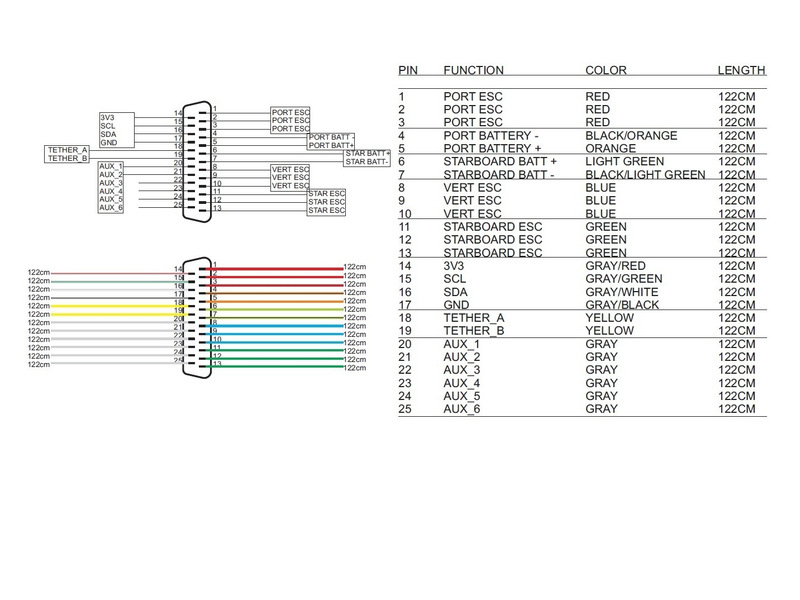
\includegraphics[width=12cm]{img/cap3/3_5/DB-25}
\end{center}
\caption{DB-25}
\label{fig:db25}
\end{figure}

\newpage

\item \textbf{Enredos}.

Facilmente el robot puede quedar atrapado en el suelo oceánico por culpa de las algas u otros objetos o vegetales.

Lo mejor es evitar pilotar el robot en un paisaje con una vegetación pesada.

Si comprobamos que no se puede sacar el OpenROV por medio de los comandos, tiraremos de la correa hasta la superficie. Aunque puede existir un momento en el que el robot no pueda ser recuperado por ese medio, en ese caso, se puede cortar la correa e ir a buscar al robot, ya que se puede volver a soldar la correa.

\item \textbf{Inundación del tubo principal}.

El mayor problema al que nos podemos enfrentar, es que se inunde el tubo principal, que conllevaría al riesgo de perder el hardware del robot.

Primero, se desconecta la alimentación del robot desenchufando el cable USB y seguidamente retiraremos las baterías.

Enjuagamos los componentes electrónicos que se mojaron en el agua para eliminar los residuos del hardware, desmontaremos los componentes electrónicos y volveremos a enjuagar.

Secaremos bien cada una de las piezas de la electrónica. Lo más recomendable es usar una pistola de aire comprimido.

Para finalizar, se colocaran todos los componentes electrónicos afectados en un lugar seco. Lo mejor es usar una bolsa de llena de arroz.

Cuando se vuelve a montar el robot, verificaremos que no exista corrosión. Si la hubiera, se intentará eliminar con un cepillo.
\end{enumerate}


% Capitulo 4
\chapter{Integración de ROS en OpenROV}
\label{cap:integracionROS}

En este capítulo se va a describir como se ha realizado la integración de ROS con OpenROV\cite{ros_rov}.

Para ello, utilizaremos las bibliotecas de ROS Rosbridge y Roslibjs, que nos proporcionarán la comunicación entre el ordenador y el robot OpenROV.

\section{Configuración del ROV}
\label{cap:Configuracion del ROV}
La electrónica de OpenROV se basa en un Arduino conectado a una placa BeagleBone, que ejecutará el software de OpenROV.

Para la implementación de ROS con OpenROV se ha decidido implementar ROS en el portátil en lugar de en el ROV, ya que se necesita ejecutar un ROS Master. Si se hubiera realizado a la inversa, se necesitaría acceso al robot para ejecutar el ROS Master, por lo que una vez sumergido no podríamos utilizar ROS.

El ROS Master se ejecutará en el portátil y será el que interactue con los nodos de ROS instalados, en este caso, Rosbridge.

Para la comunicación de ROS y OpenROV usaremos el paquete Roslibjs el cual instalaremos dentro del software del robot. Roslibjs es la biblioteca que utiliza JavaScript para comunicarse con ROS. Roslibjs publicará y/o suscribirá a los mensajes de ROS.

Se utilizará el paquete de Rosbridge para traducir los mensajes JSON en mensajes ROS (OpenROv utiliza JSON para su comunicación). Este paquete actúa como un Nodo de ROS que puede publicar y/o suscribir a los mensajes.

En conclusión, la comunicación se realizara a través de una conexión Websocket (Rosbridge) y el paquete de Roslibjs.

La figura a continuación muestra la estructura básica de ROS para la integración de OpenROV.

\begin{figure} [hbtp]
  \begin{center}
    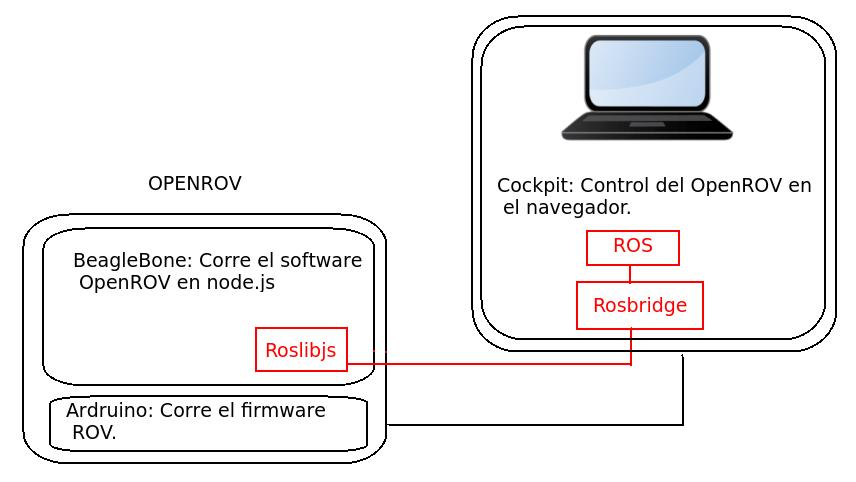
\includegraphics[width=8cm]{img/cap4/conect_ros_rov}
  \end{center}
  \caption{Diagrama de la conexión ROS y OpenROV}
  \label{fig:conect_ros_rov}
\end{figure}

Para configurar el robot se debe instalar el Roslibjs, sin embargo, este paquete necesita de varias dependencias.

Comenzaremos configurando el BeagleBone a través de una conexión SSH, conectando un cable Ethernet entre el BeagleBone y el router.
Para activar el hardware usaremos un cable miniUSB conectado entre el BeagleBone y el portátil.
Una vez realizadas las conexiones, haremos un SSH a la placa.
\renewcommand{\lstlistingname}{}
\begin{lstlisting}[caption=SSH, label={lst:ssh}]
$ ssh rov@192.168.7.2
\end{lstlisting}
cuando pida la contraseña, deberemos introducir “OpenROV”.

\begin{figure} [hbtp]
  \begin{center}
    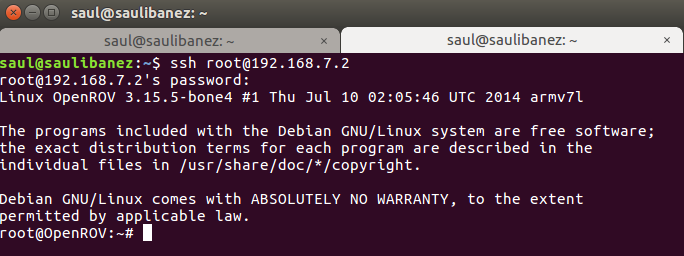
\includegraphics[width=12cm]{img/cap4/ssh}
  \end{center}
  \caption{SSH}
  \label{fig:ssh}
\end{figure}

Para instalar las dependencias de Roslibjs, ejecutaremos los siguientes comandos:

\renewcommand{\lstlistingname}{}
\begin{lstlisting}[caption=Dependencias Roslibjs, label={lst:roslibjs}]
sudo apt-get update 
sudo apt-get install libcairo2-dev libjpeg-dev libpango1.0-dev libgif-dev build-essential g++
\end{lstlisting}

\begin{figure} [hbtp]
  \begin{center}
    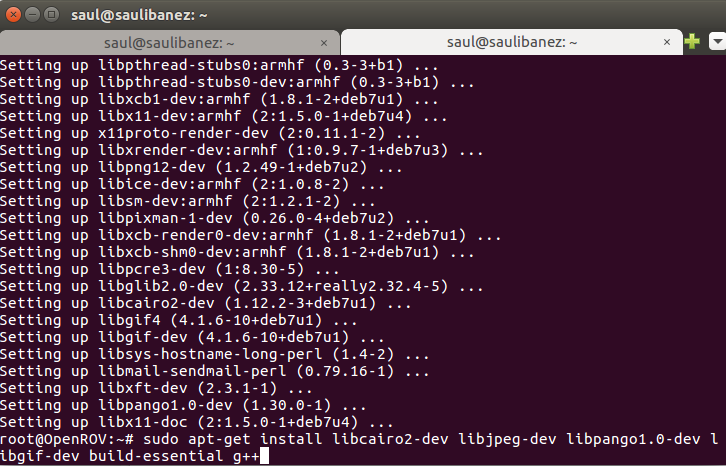
\includegraphics[width=12cm]{img/cap4/dependencias_roslibjs}
  \end{center}
  \caption{Dependencias Roslibjs}
  \label{fig:Dependencias Roslibjs}
\end{figure}
\newpage
Continuaremos instalando otras dependencias de Roslibjs, en este caso, npm, que es un gestor de paquetes que utiliza Node.js.
\\Para que no surjan errores con el proxy, debemos deshabilitarlo y realizar un reseteo del sistema. 
\renewcommand{\lstlistingname}{}
\begin{lstlisting}[caption=Dependencias Roslibjs, label={lst:roslibjs}]
$ sudo /etc/init.d/openrov-proxy stop
$ sudo /etc/init.d/openrov restart
$ sudo chown -R $USER /usr/local 
$ npm install canvas 
\end{lstlisting}

\newpage
\begin{figure} [hbtp]
  \begin{center}
    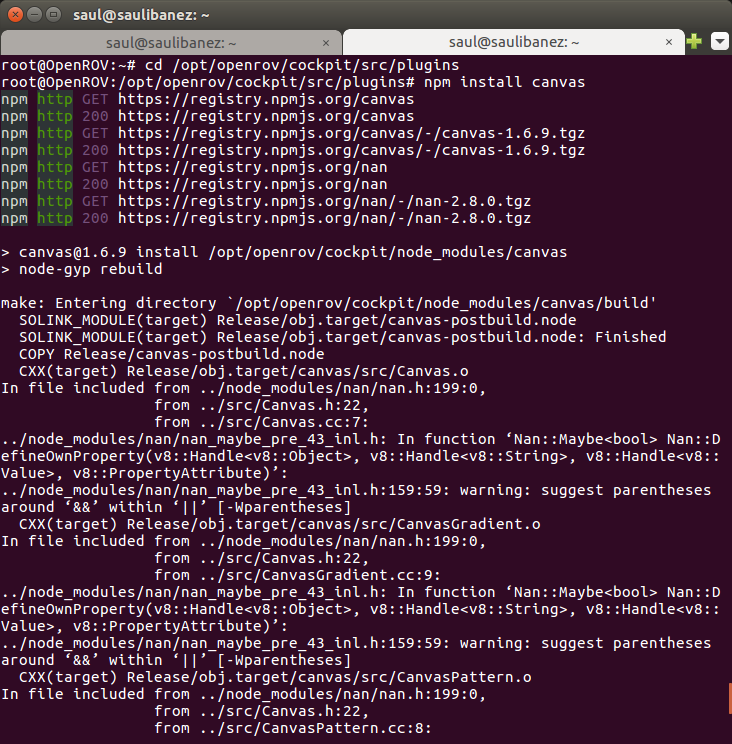
\includegraphics[width=12cm]{img/cap4/canvas}
  \end{center}
  \caption{Canvas}
  \label{fig:canvas}
\end{figure}

La última dependencia para el complemento es Roslibjs, lo instalaremos usando: 
\renewcommand{\lstlistingname}{}
\begin{lstlisting}[caption=Roslib, label={lst:roslib}]
$ npm install roslib
\end{lstlisting}

Dentro de la carpeta /opt/openrov/cockpit/src/plugins, creararems un directorio llamado ros (sudo mkdir ros) y en el, se creará un fichero llamado index.js, que ejecutará la conexión con el ROS Master localizado en el portátil.
\newpage
\renewcommand{\lstlistingname}{}
\begin{lstlisting}[caption=Conexión con ROS, label={lst:conection_ros}]
function ros(name, deps) {
  		console.log("ROS plugin started");

  		// Comienza la sesion de ROS
 		var ROSLIB = require("roslib")
  		var ros = new ROSLIB.Ros({
    			url : 'ws://192.168.7.1:9090'
  		});

  		ros.on('connection', function() {
   			console.log('ROS connected to websocket');
  		});

  		ros.on('error', function(error) {
    			console.log('ROS error connecting to websocket');
  		});

 		 ros.on('close', function() {
    			console.log('ROS closed websocket connection');
 		});
	};

	module.exports = ros;
\end{lstlisting}

También se debe modificar el fichero hosts (sudo vim /etc/hosts) y en el realizaremos los siguientes cambios:

\begin{lstlisting}[caption=/etc/hosts, label={lst:hosts}]
#127.0.1.1	OpenROV
192.168.7.2	OpenROV
192.168.7.1	saul.ibanez.local
\end{lstlisting}

\section{Configuración de ROS}
\label{cap:Configuracion de ROS}
Para la conexión con ROS, se decide instalar ROS Kinetic en el portátil:

\begin{lstlisting}[caption=Instalacion de ROS, label={lst:install_ros}]
sudo sh -c 'echo "deb http://packages.ros.org/ros/ubuntu $(lsb_release -sc) main" > /etc/apt/sources.list.d/ros-latest.list'
sudo apt-key adv --keyserver hkp://ha.pool.sks-keyservers.net:80 --recv-key 421C365BD9FF1F717815A3895523BAEEB01FA116
sudo apt-get update
sudo apt-get install ros-kinetic-desktop-full
apt-cache search ros-kinetic
sudo rosdep init
rosdep update
echo "source /opt/ros/kinetic/setup.bash" >> ~/.bashrc
source ~/.bashrc
sudo apt-get install python-rosinstall python-rosinstall-generator python-wstool build-essential
\end{lstlisting}

Instalaremos Rosbridge
\begin{lstlisting}[caption=Rosbridge, label={lst:rosbridge}]
sudo apt-get install ros-kinetic-rosbridge-server
\end{lstlisting}

Cuando se configuró ROS, creamos una carpeta llamada catkin\_ws, en ella, se creó también la carpeta src, en la que crearemos el directorio openrov el que debe contener un fichero CMakeLists.txt

El archivo CMakeLists.txt es la entrada al sistema de compilación CMake. El código será:

\begin{lstlisting}[caption=CMakeLists.txt, label={lst:cmakelists}]
cmake_minimum_required(VERSION 2.8.3)
project(openrov)

find_package(catkin REQUIRED COMPONENTS
  	roscpp
  	rospy
  	std_msgs
 	sensor_msgs
  	geometry_msgs
  	message_generation
)

add_message_files(
    	FILES
    	navdata.msg
    	rovstatus.msg
   	motortarget.msg
  )

add_service_files(
    FILES
)

generate_messages(
	DEPENDENCIES
    	std_msgs
    	sensor_msgs
    	geometry_msgs
)

catkin_package(
   	INCLUDE_DIRS include
   	LIBRARIES openrov
   	CATKIN_DEPENDS roscpp rospy message_runtime
                  std_msgs sensor_msgs geometry_msgs
   	DEPENDS system_lib
)

include_directories(
  	${catkin_INCLUDE_DIRS}
)
\end{lstlisting}


Además, crearemos un directorio nombrado launch en el que se creará el fichero rosbridge.launch:

\begin{lstlisting}[caption=websocket.launch, label={lst:launch}]
<launch>
 	<include file="$(find rosbridge_server)/launch/rosbridge_websocket.launch"/>
</launch>
\end{lstlisting}

Este código conduce a la instalación de rosbridge\_server e iniciará la conexión con ROV.

Para finalizar, y antes de ejecutar el .launch, deberemos ejecutar otro fichero, llamado set\_remote\_robot, el cual está configurado de la siguiente manera:
\begin{lstlisting}[caption=set\_remote\_robot, label={lst:remote}]
	export ROS_IP=192.168.7.1 	#YOUR IP
	export ROS_HOSTNAME=saulibanez.local 	#YOUR MACHINE
	export ROS_MASTER_URI=http://saulibanez.local:11311
\end{lstlisting}

\section{Conexión de ROS en OpenROV}
\label{cap:Conexion de ROS en OpenROV}

Habiendo realizado todos los pasos anteriores, ya estamos preparados para realizar la conexión de ROS en OpenROV.

Empezaremos conectando el OpenROV (solo con el cable MiniUSB en el portátil) abriremos un terminal y realizaremos un SSH a el BeagleBone (ssh rov@192.168.7.2).

Una vez conectados, desactivaremos el proxy (sudo /etc/init.d/openrov-proxy stop) y reinicamos elrobot (sudo /etc/init.d/openrov restart).

En otro terminal, ejecutaremos un roscore, que iniciará el ROS Master.

\begin{figure} [hbtp]
  \begin{center}
    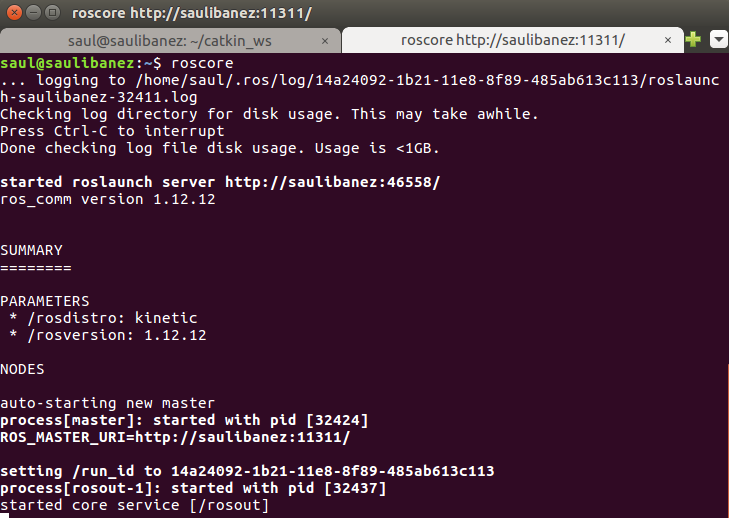
\includegraphics[width=11cm]{img/cap4/roscore}
  \end{center}
  \caption{Roscore}
  \label{fig:roscore}
\end{figure}
\newpage

Continuaremos lanzando el programa rosbridge.launch, que inciará el nodo de rosbridge para comunicare con el robot.

Ejecutando el código:
\begin{lstlisting}[caption=launch, label={lst:launch}]
	$ roslaunch openrov rosbridge.launch
\end{lstlisting}

\begin{figure} [hbtp]
  \begin{center}
    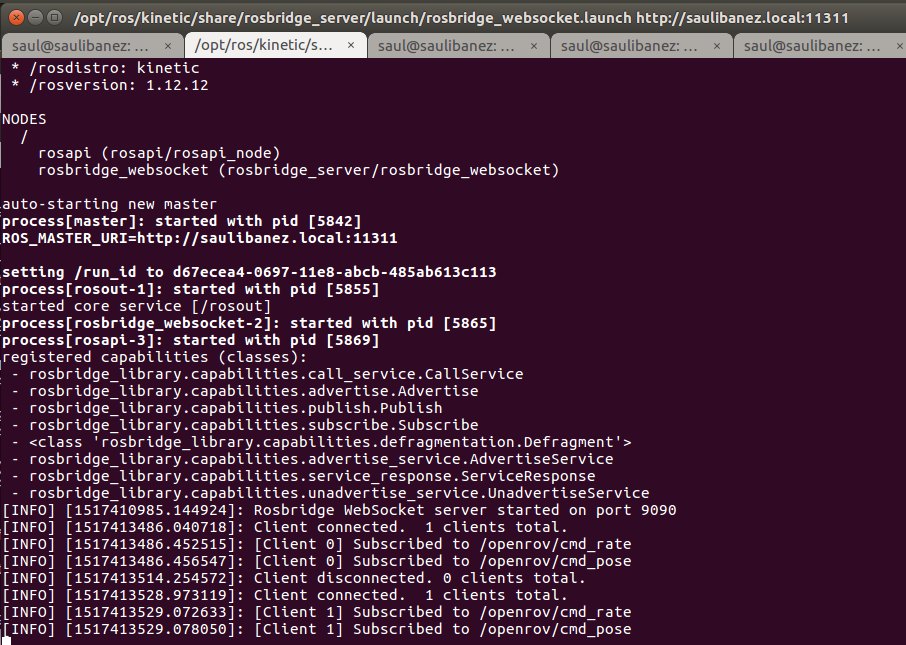
\includegraphics[width=11cm]{img/cap4/launch}
  \end{center}
  \caption{Launch}
  \label{fig:websocket.launch}
\end{figure}

También se comprobará en el terminal de OpenROV que la conexión se ha realizado

\begin{figure} [hbtp]
  \begin{center}
    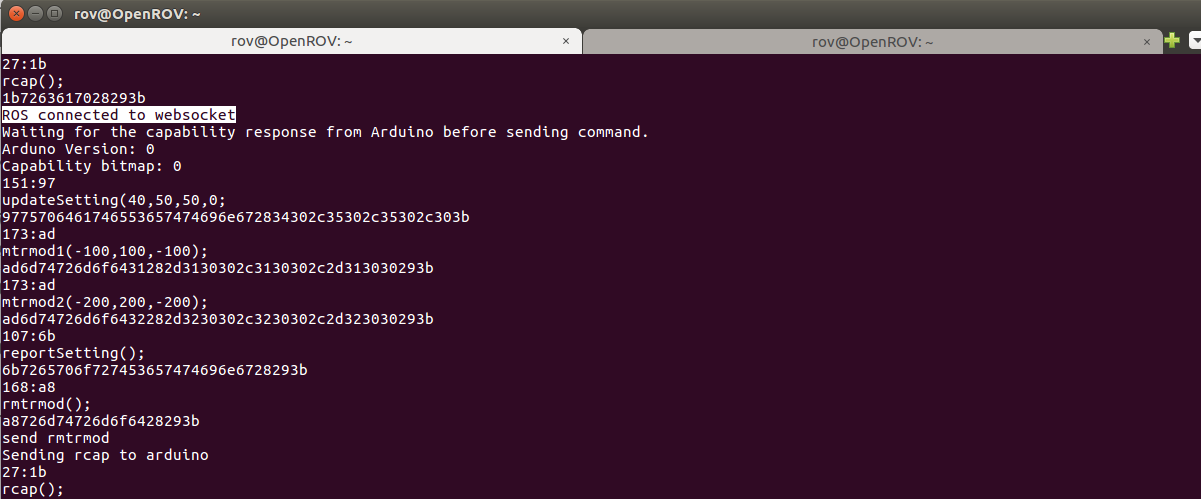
\includegraphics[width=12cm]{img/cap4/conexion_ROV}
  \end{center}
  \caption{Conexión en ROV}
  \label{fig:conect_rov}
\end{figure}

Para asegurarse de que todo esté funcionando, abrimos otra pestaña en el terminal e ingresaremos:
\begin{lstlisting}[caption=rostopic list, label={lst:list}]
	$ rostopic list
\end{lstlisting}

Esto mostrará una lista de los temas que están siendo publicados por el ROV, así como algunos temas predeterminados.

\begin{figure} [hbtp]
  \begin{center}
    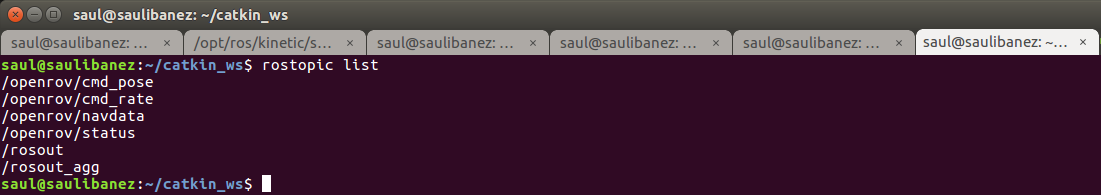
\includegraphics[width=12cm]{img/cap4/rostopic_list}
  \end{center}
  \caption{rostopic list}
  \label{fig:rostopic_list}
\end{figure}

Para ver información sobre el nodo en particular podremos ejecutar el comando: rostopic info.
\begin{lstlisting}[caption=rostopic info, label={lst:info}]
	$ rostopic info
\end{lstlisting}

\begin{figure} [hbtp]
  \begin{center}
    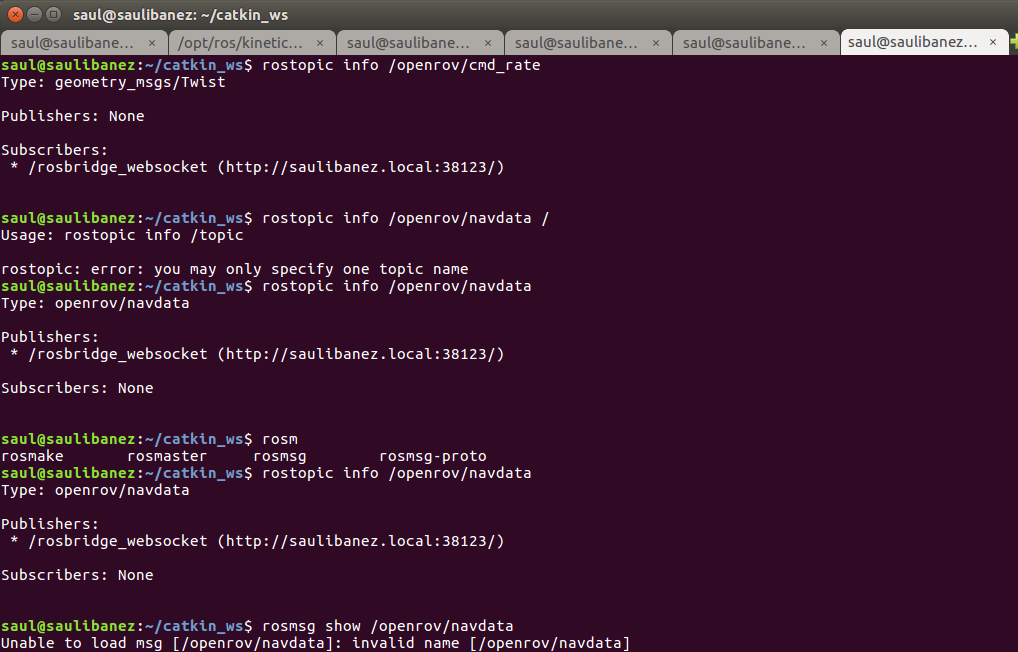
\includegraphics[width=12cm]{img/cap4/info1}
  \end{center}
  \caption{rostopic info (1)}
  \label{fig:rostopic_info}
\end{figure}
\begin{figure} [hbtp]
  \begin{center}
    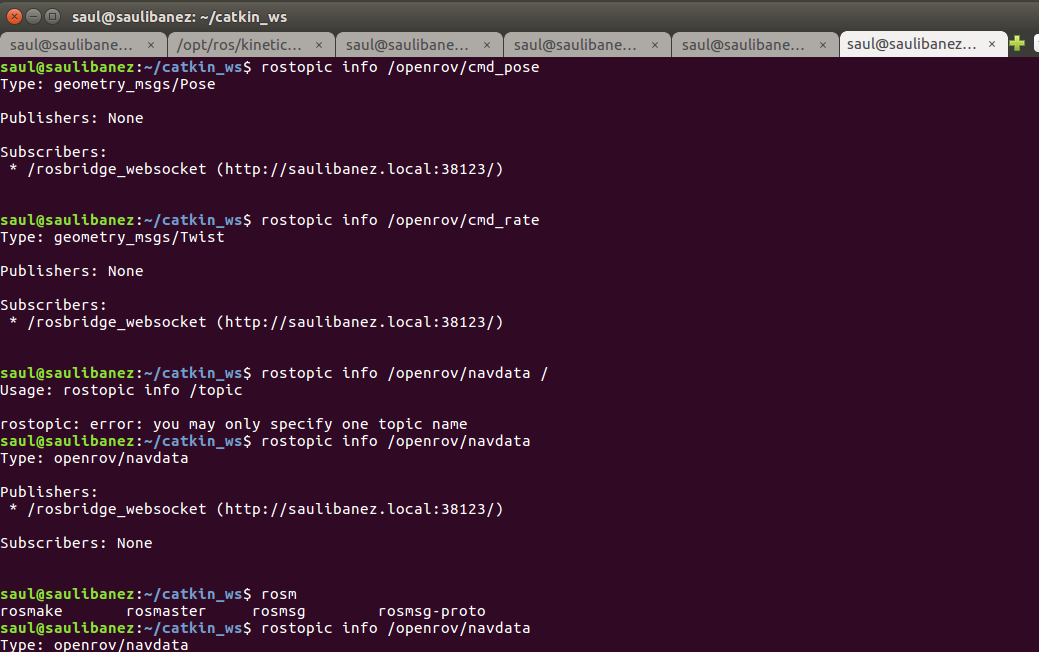
\includegraphics[width=12cm]{img/cap4/info2}
  \end{center}
  \caption{rostopic info (2)}
  \label{fig:rostopic_info}
\end{figure}

% Capitulo 5
\chapter{Pruebas de Campo}

En este capitulo, se adjuntarán unos vídeos comprobando el funcionamiento del robot.

\begin{enumerate}
\item En el primer vídeo, después de haber realizado la soldadura de los motores y comprobado que existe conectividad, se verifica que su funcionamiento es el adecuado.
 
https://www.youtube.com/watch?v=pck8Bpla-5w
 
 \begin{figure} [hbtp]
  \begin{center}
    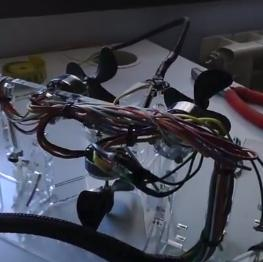
\includegraphics[width=7cm]{img/cap5/motores}
  \end{center}
  \caption{Prueba de motores}
  \label{fig:motores}
 \end{figure}

\item Una vez montado el robot, antes de llevarlo al exterior, se comprueba que es estanco y que el hardware no sufre ningún daño, para este proceso, llenamos la bañera de agua e introducimos el robot.
 
También se comprueba que funcionan todas las aplicaciones instaladas y que puede permanecer más de 6 horas bajo el agua sin incidentes.

https://www.youtube.com/watch?v=jqZOBc\_-mvU
\newpage
 \begin{figure} [hbtp]
  \begin{center}
    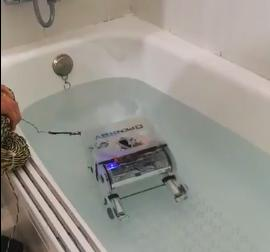
\includegraphics[width=7cm]{img/cap5/banera}
  \end{center}
  \caption{Prueba de funcionamiento en la bañera}
  \label{fig:banera}
 \end{figure}
 


\item Una vez comprobados los dos apatados anteriores, es momento de comprobar su funcionamiento en un entorno más hostil, para ello, nos hemos dirigido a un lago.
 
Antes de sumergirlo, comprobaremos que todo funciona correctamente y que no se necesita internet para interactuar con el robot.

https://www.youtube.com/watch?v=0LhODkpdkcw

 \begin{figure} [hbtp]
  \begin{center}
    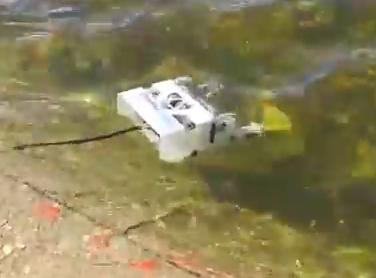
\includegraphics[width=7cm]{img/cap5/lago1}
  \end{center}
  \caption{Prueba de funcionamiento en el lago}
  \label{fig:lago}
 \end{figure}
 

\newpage
\item En este video, se comprueba que el robot puede navegar por el lago sin ningún problema.
 
https://www.youtube.com/watch?v=KLFG9klwu\_Q
 
 \begin{figure} [hbtp]
  \begin{center}
    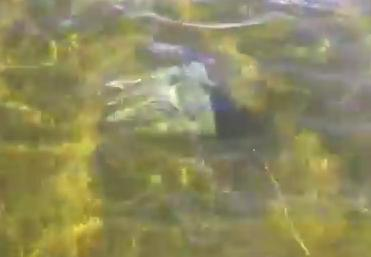
\includegraphics[width=7cm]{img/cap5/navegacion}
  \end{center}
  \caption{Prueba de navegación en el lago}
  \label{fig:navegacion}
 \end{figure}

\item Se realiza una prueba de emersión para comprobar que el robot puede volver a la superficie sin problemas.

https://www.youtube.com/watch?v=Q6qG2w9rGW0

 \begin{figure} [hbtp]
  \begin{center}
    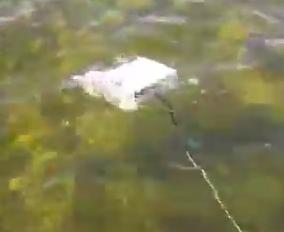
\includegraphics[width=7cm]{img/cap5/emersion}
  \end{center}
  \caption{Prueba de emersión del lago}
  \label{fig:emersion}
 \end{figure}

\newpage
\item En el último video, vemos gracias a la web, todo lo que el robot esta visualizando en el fondo del lago.
 
https://www.youtube.com/watch?v=svbzpc0WSwE
 
 \begin{figure} [hbtp]
  \begin{center}
    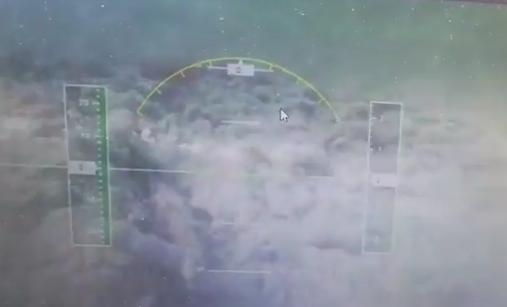
\includegraphics[width=7cm]{img/cap5/web}
  \end{center}
  \caption{Prueba de visualización del lago en la web}
  \label{fig:web}
 \end{figure} 


\end{enumerate}

% Capitulo 6
\chapter{Conclusiones}
\label{cap:conclusiones}

Los objetivos de este trabajo de fin de grado han sido dos. Por un lado, presentar a los robots submarinos, en particular, OpenROV, y por otro lado, la integración de ROS, el framework de robótica más extendido y utilizado con la tecnología del ROV.

Al realizar todo el montaje y la configuración desde cero, he podido conocer amplios aspectos acerca de la tecnología del ROV, además de explorar los paquetes necesarios de ROS para realizar la comunicacion entre ROS y OpenROV.

Tras finalizar el montaje y el sistema del OpenROV, aprendí a solventar imprevistos que no se contemplaban, tanto de hardware como de software. En este aspecto, la comunidad de OpenROV ha sido de inestimable ayuda en algunos momentos.

Se comprobó que el robot es estanco y puede navegar bajo la superficie marina, que todos los controles mencionados en los puntos anteriores funcionan correctamente (láser, cámara, luces, etc) y que pueden aparecer algunos de los problemas comunes (por ejemplo, el vaho).

Debido a que OpenROV tiene software libre, se pudo instalar los paquetes necesarios para realizar la comunicación con ROS y se comprobó que existía la comunicación entre las dos plataformas. 

Se podrían mejorar ciertos aspectos del OpenROV si se siguen implementando nodos de ROS para su utlilización. Por ejemplo, para la cámara podría usarse el paquete sensors; para la velocidad podría utilizarse geometry\_msgs; etc. 

Para finalizar, otro de los siguientes hitos que se podrían realizar con este TFG es intentar descubrir si la leyenda de Nessie es cierta.


%Te recomiendo leer \cite{openrov, ros, RoboticaMovil, cascada, ros_rov, telemetria}.

%bibliografia
\bibliographystyle{IEEEannot}
\bibliography{bibliografia}


\end{document}
